\chapter{Airplanes}

A loaded Boeing 747 weighs about 400,000 kg, as much as 300 cars. Yet it
lifts off the runway and cruises at 900 km per hour. In this chapter, you will see how.
Good news: if you understood how a sail works, you already understand
most of an airplane.

\section{Drag and Thrust}

As an airplane flies, the air pushes back on it, trying to slow it down.
Pilots call this force \newterm{drag}\index{drag}. You can think of drag as
air friction.

Drag grows with the square of the speed. Double your speed, and the drag
becomes four times as large. (You have felt this: stick your hand out of a
car window at 30 km/h, then at 60 km/h.)

To overcome drag, an airplane needs \newterm{thrust}\index{thrust}, a
forward push. Airplanes get thrust by throwing air toward the back of the
plane. By Newton's third law, the air pushes the plane forward.

All that pushing takes a lot of fuel. A Boeing 747 burns about 4 liters of
fuel every second, and a flight from London to New York needs about
70,000 kg of it. At takeoff, the fuel can weigh nearly twice as much as all
the passengers.

\section{Lift}

A hot air balloon floats because it is lighter than the air it displaces.
An airplane is far heavier than the air it displaces, so gravity would pull
it from the sky without another upward force. That force is
\newterm{lift}\index{lift}.

Lift works just like sailing on a close reach. The wing meets the air at a
slight tilt, its \index{angle of attack}\newterm{angle of attack}. Air
piles up under the wing, creating high pressure. Air flowing smoothly over
the curved top of the wing leaves low pressure there. The difference in
pressure pushes the wing up. A shape designed to do this is called an
\newterm{airfoil}\index{airfoil}. Wings, propeller blades, kites, and sails
are all airfoils.

\begin{figure}[H]
    \centering
    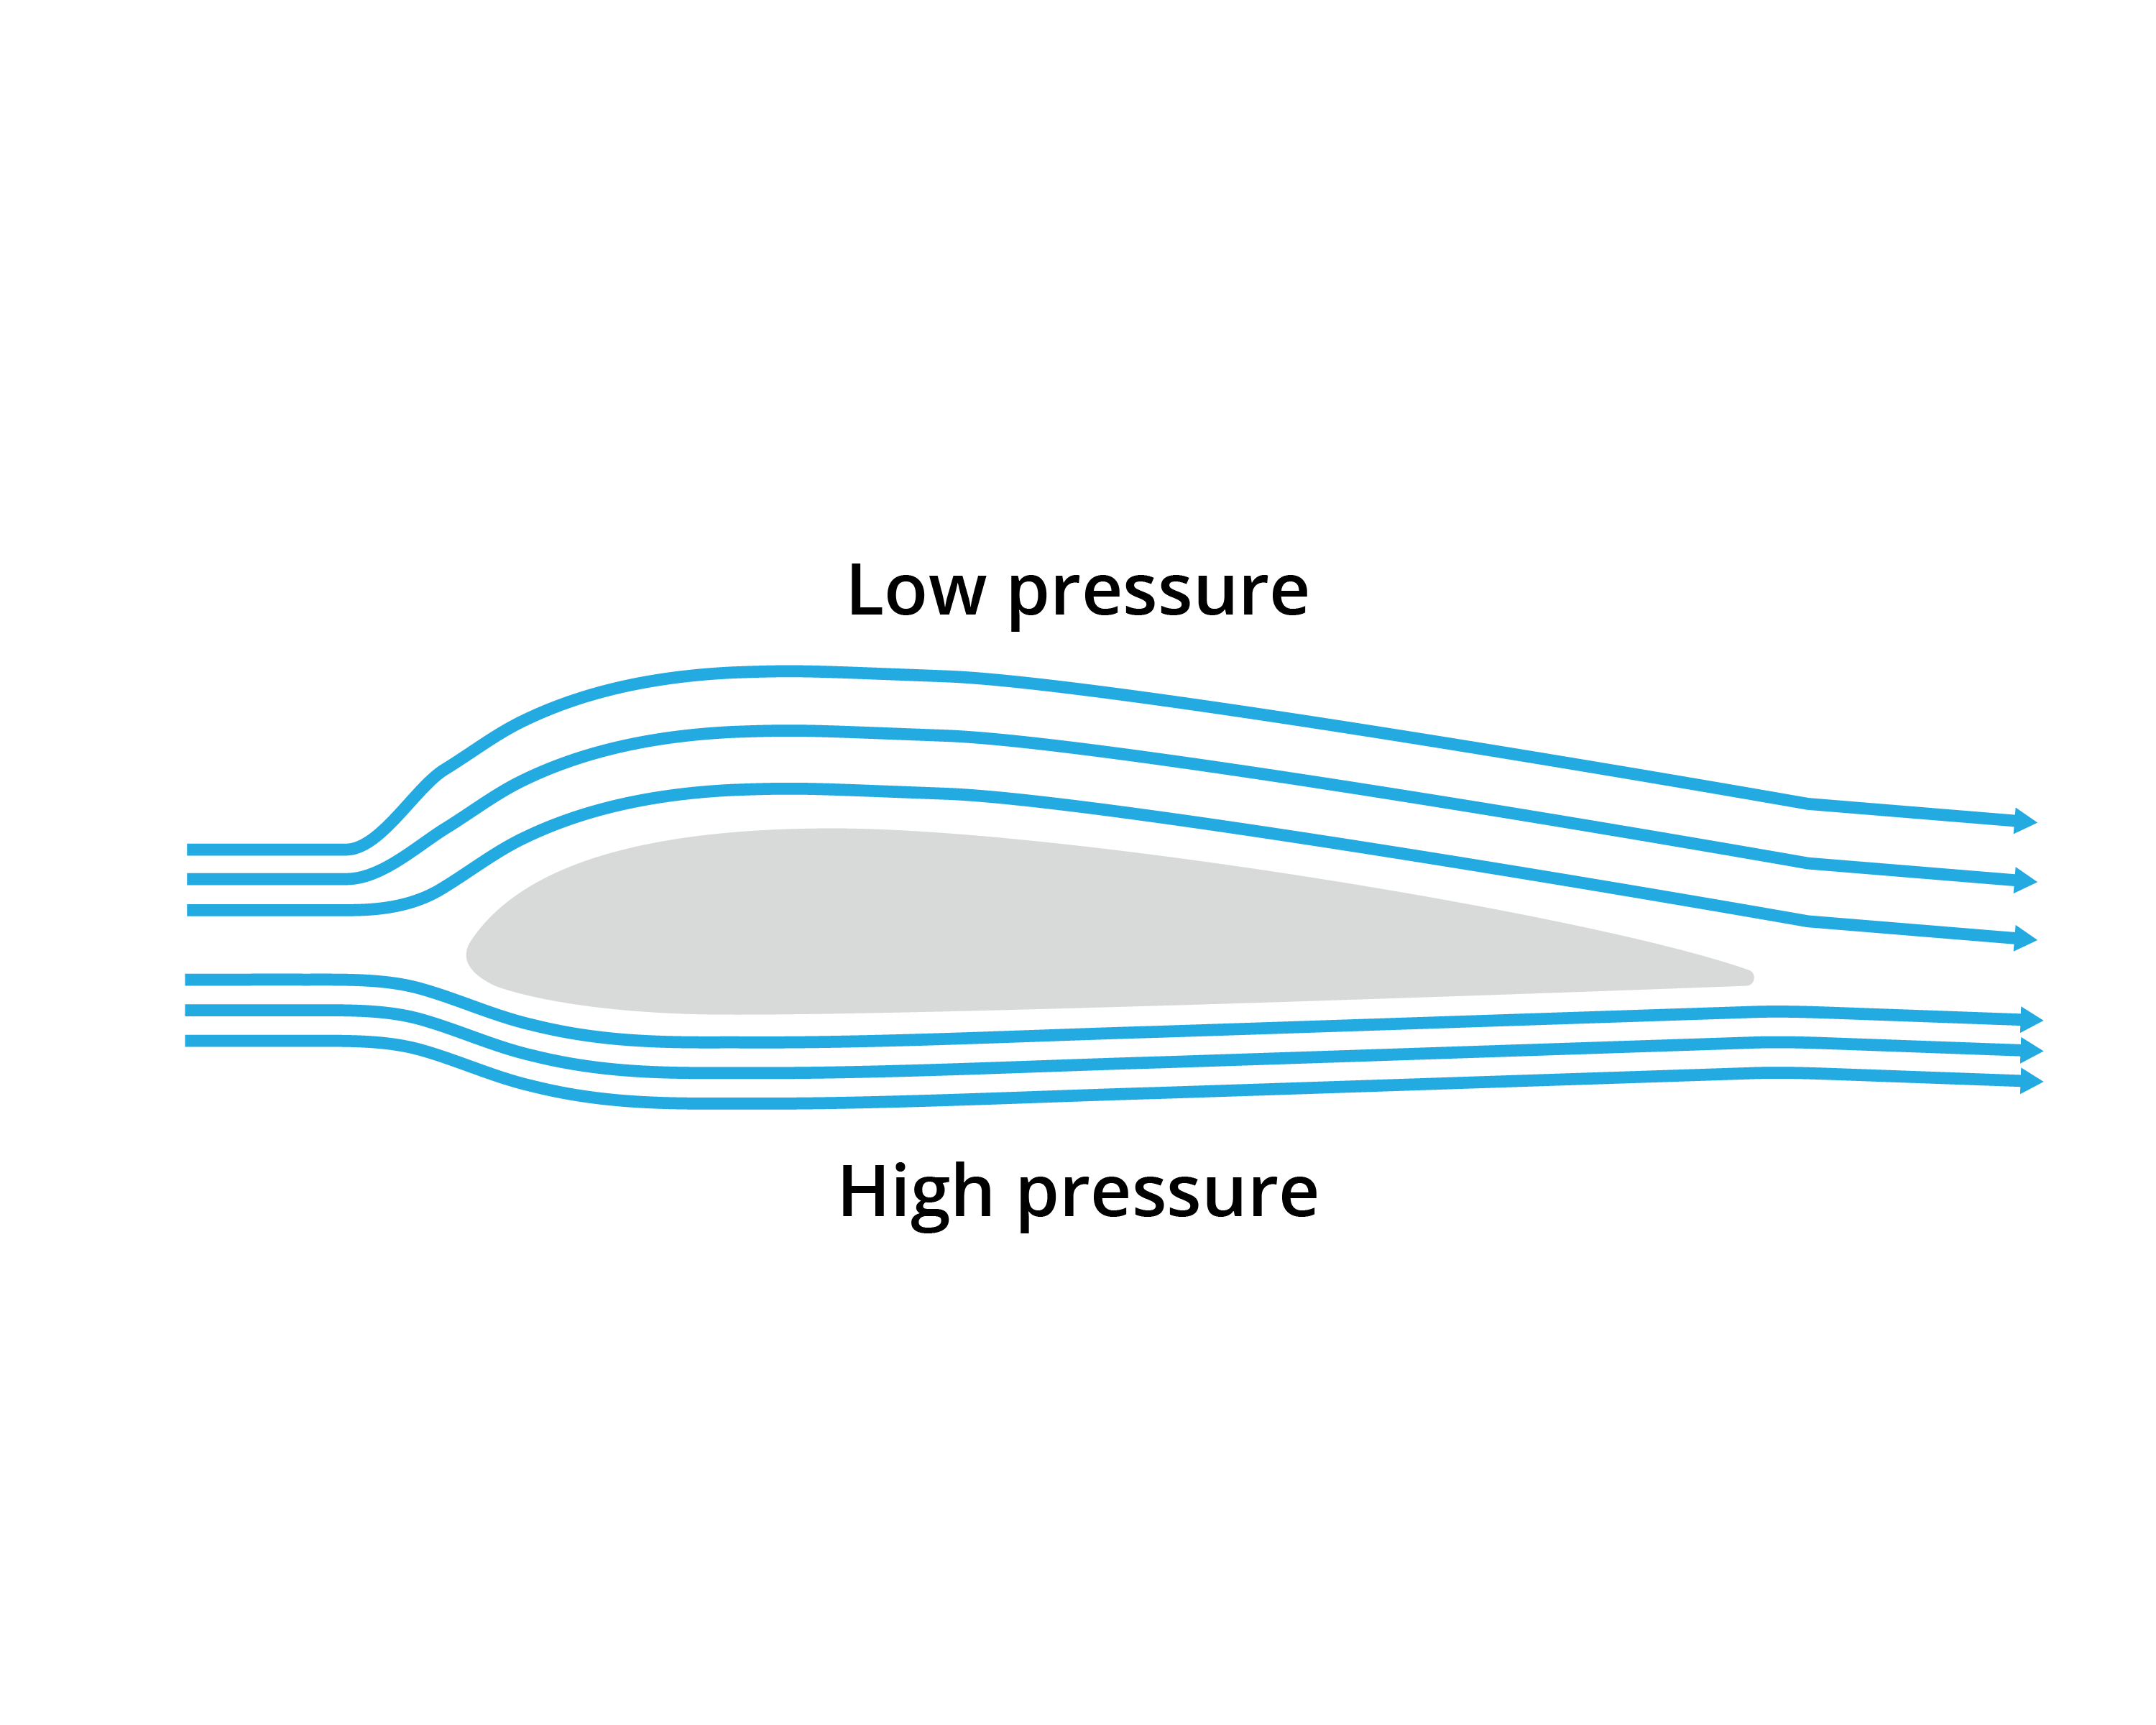
\includegraphics[width=0.55\textwidth]{airfoil.png}
    \caption{Air flowing around a wing. The wing deflects air downward,
    leaving high pressure below and low pressure above.}\label{fig:airfoil}
\end{figure}

\begin{figure}[H]
    \centering
    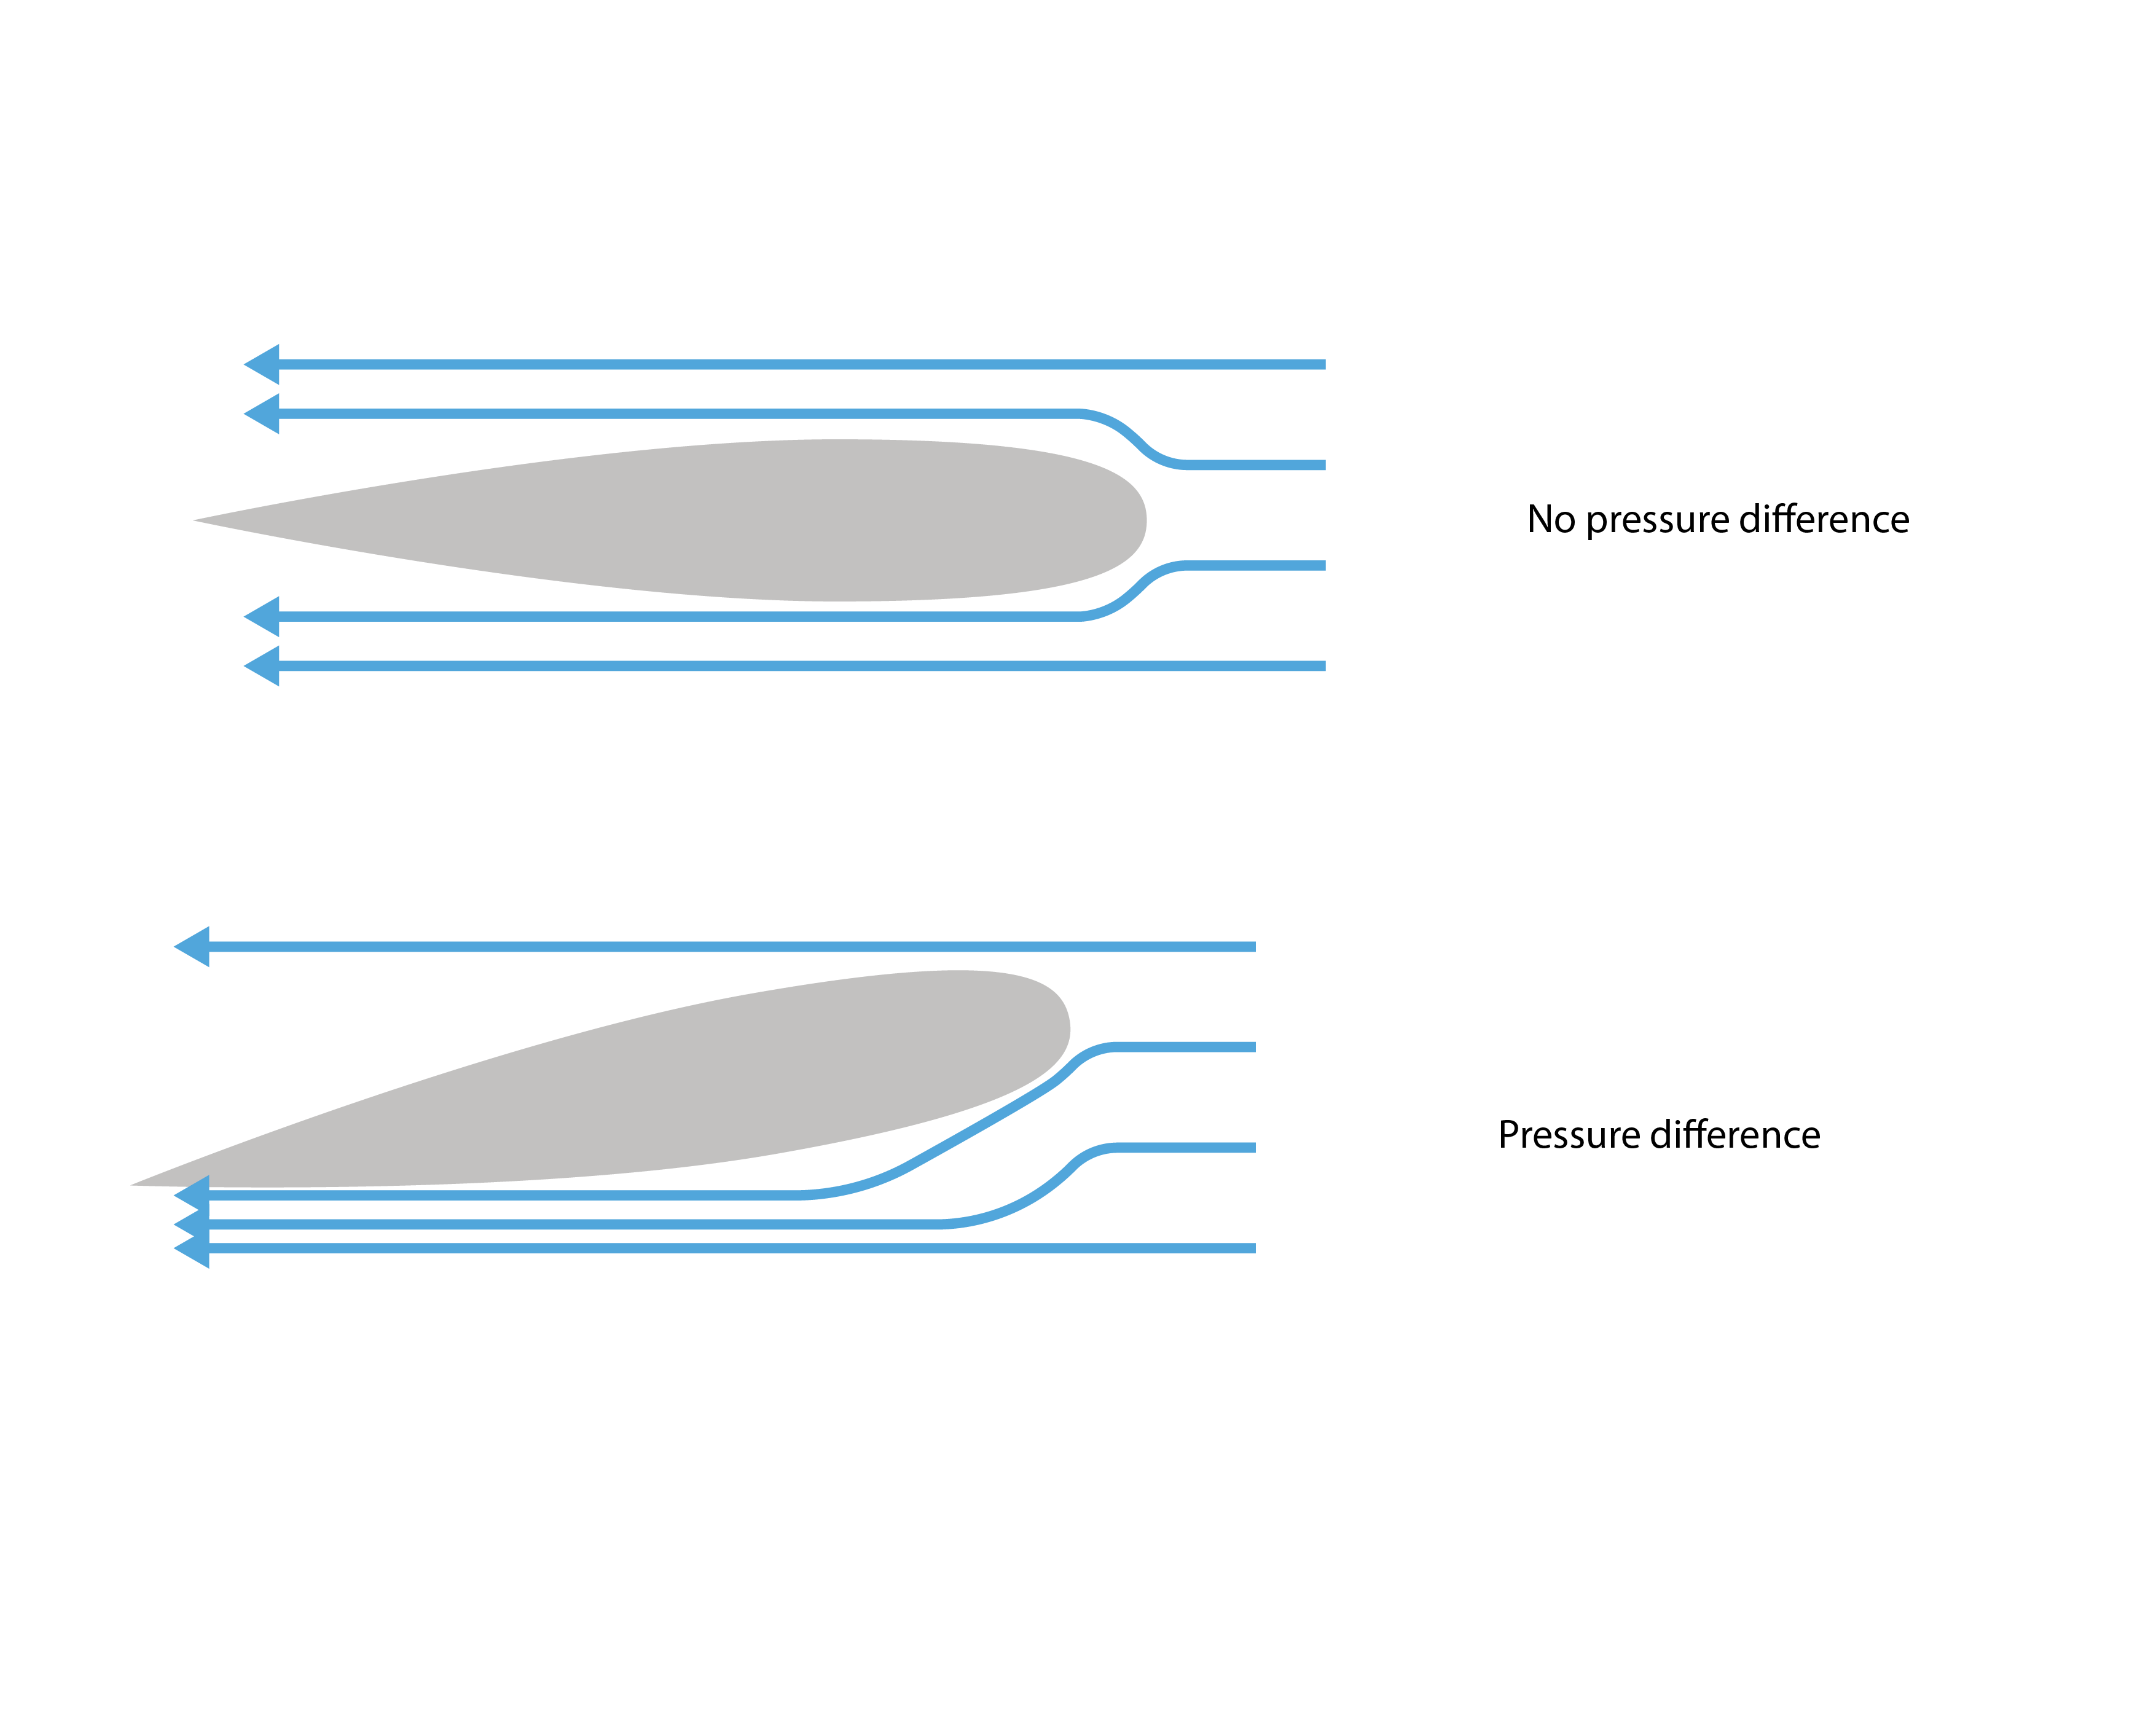
\includegraphics[width=0.8\textwidth]{pitchChange.png}
    \caption{A symmetric airfoil meeting the air head-on (top) creates no
    pressure difference. Tilted to an angle of attack (bottom), it does.}
    \label{fig:example-flight}
\end{figure}

You may have heard that lift comes mostly from the rounded top of the
wing. That explanation oversells the curve. Stunt planes fly upside down
for minutes at a time, which would be impossible if the curved top did all
the work. The angle of attack matters most; the curve helps the air stay
smoothly attached to the wing.

Engineers capture all of this in the \newterm{lift equation}:
$$L = \frac{1}{2}\rho v^2 S C_L$$
where $\rho$ is the density of the air, $v$ is the airspeed, $S$ is the
wing area, and $C_L$ is the \newterm{lift coefficient}, a number that
depends on the wing's shape and angle of attack. Notice the
$\frac{1}{2}\rho v^2$: it is exactly the wind pressure from the sailing
chapter, which the Fluids in Motion chapter called the dynamic pressure. That
chapter also explains how Bernoulli's equation and Newton's third law describe
the same lift.

\textbf{Worked example.} A small plane has a wing area of 20 m$^2$ and
flies at 50 m/s through air with $\rho = 1.2$ kg/m$^3$. Its lift
coefficient is 0.5. How much lift do the wings produce?

\textbf{Solution.}
$L = \frac{1}{2}(1.2)(50)^2(20)(0.5) = 15{,}000$ N. That is enough to hold
up about $\frac{15{,}000}{9.8} \approx 1{,}500$ kg, the mass of a small
plane with its passengers.

\begin{Exercise}[title={Doubling the Speed}, label=fl1]
Using the same wing and angle of attack, what is the lift at $100$ m/s?
\end{Exercise}
\begin{Answer}[ref=fl1]
Lift depends on $v^2$, so doubling the speed multiplies the lift by four:
$L = 60{,}000$ N.
\end{Answer}

High in the sky, the air is thinner. If two identical planes fly at the same
speed at different altitudes:
\begin{itemize}
\item The higher plane feels less drag.
\item The higher plane's wings make less lift.
\item The higher plane's engines get less oxygen per liter of air, which
      changes how the fuel burns.
\end{itemize}
Airliners cruise at about 11 km because the thin air means less drag and
better fuel economy; they make up for the weaker lift by flying fast.

\begin{Exercise}[title={Thin air}, label=fl_altitude]
At 11 km, the air density is about 0.36 kg/m$^3$. How fast must the plane
from the worked example fly to make the same 15,000 N of lift (with the
same lift coefficient)?
\end{Exercise}
\begin{Answer}[ref=fl_altitude]
Solve $15{,}000 = \frac{1}{2}(0.36)v^2(20)(0.5)$: $v^2 = \frac{15{,}000}{1.8}
\approx 8{,}333$, so $v \approx 91$ m/s. The air is one third as dense, so
the plane must fly $\sqrt{3} \approx 1.7$ times as fast.
\end{Answer}

\section{Control: Roll, Pitch, Yaw}
\index{roll}
\index{pitch}
\index{yaw}
A plane can rotate three ways. Nose up and down is \newterm{pitch}. One wing
up and the other down is \newterm{roll}. Nose left and right is
\newterm{yaw}. The pilot has a control for each.

The first control is the throttle, which sets the thrust.

The pilot also has a stick. Pulling back on the stick tilts the
\newterm{elevator}\index{elevator} on the tail up. Air hitting the elevator
pushes the tail down and the nose up. Pushing the stick forward does the
opposite. The elevator controls pitch.

\begin{figure}[H]
  \centering
  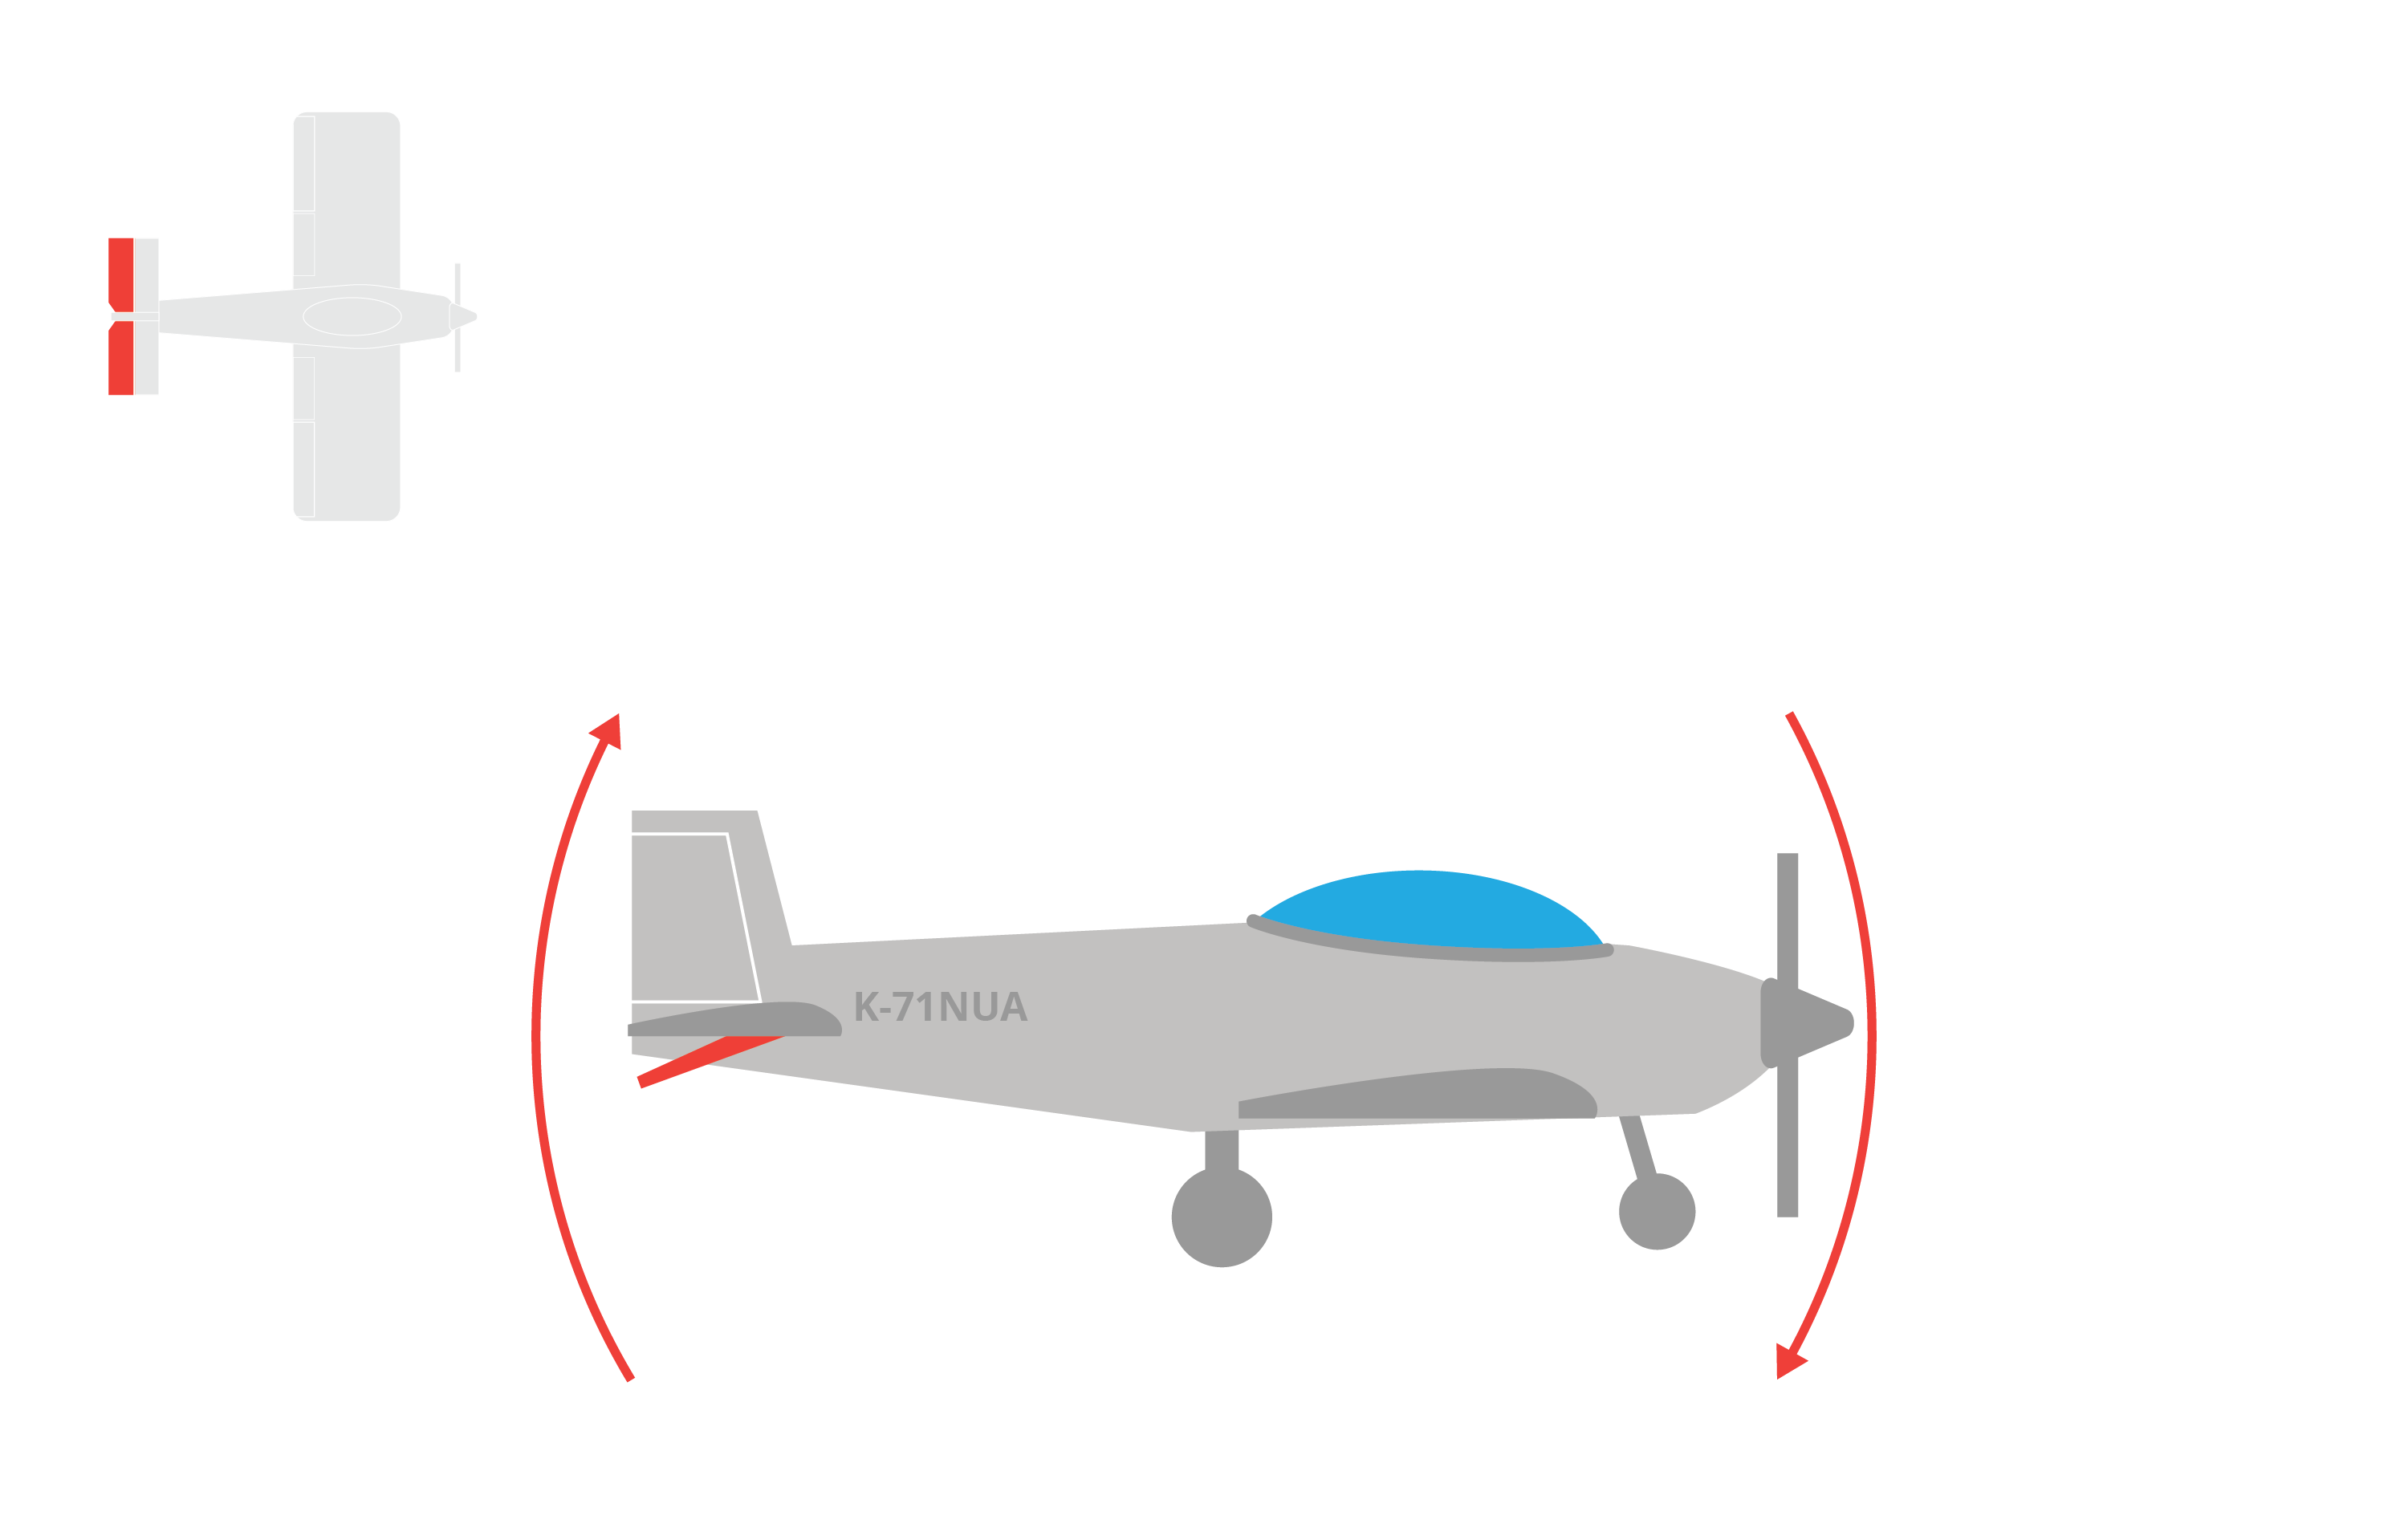
\includegraphics[width=0.55\textwidth]{elevator.png}
  \caption{Top and side views of the elevator and the pitch it produces.}\label{fig:elevator}
\end{figure}

The stick also moves left and right. Pushing it left raises the
\newterm{aileron}\index{aileron} on the left wing and lowers the aileron on
the right wing. The left wing drops and the right wing rises. The ailerons
control roll.

\begin{figure}[H]
  \centering
  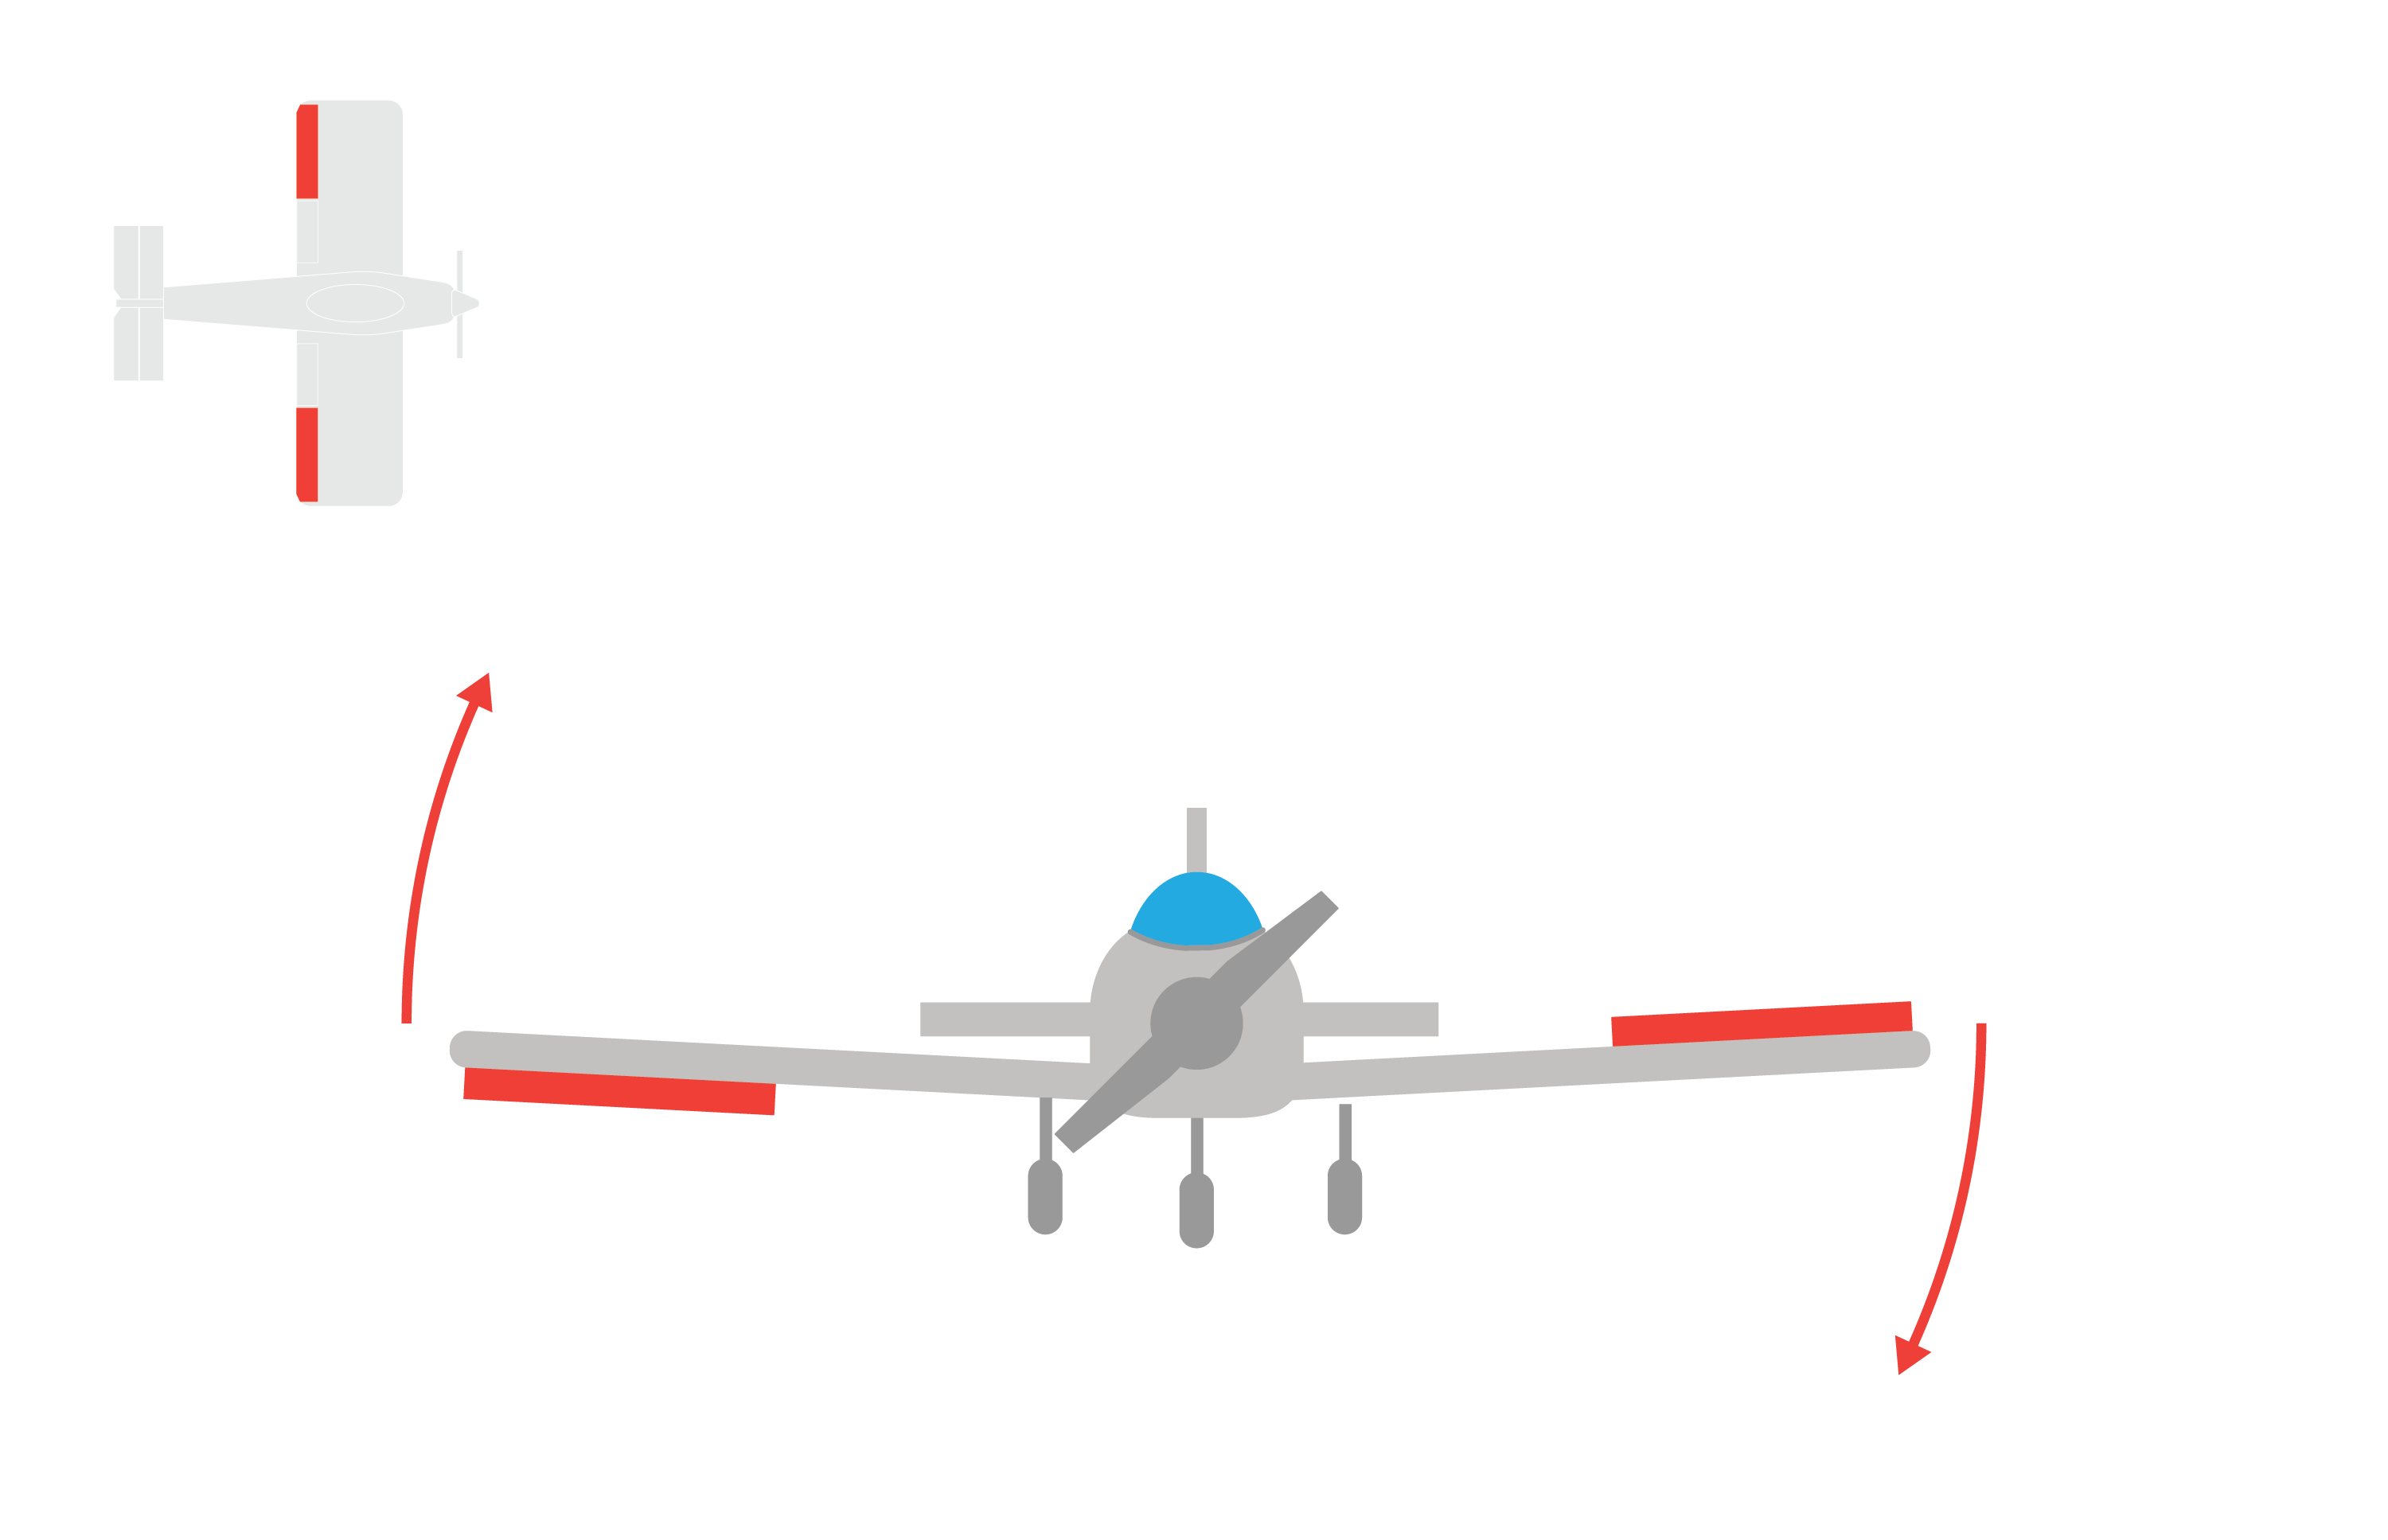
\includegraphics[width=0.55\textwidth]{ailerons.png}
  \caption{Aileron locations on the plane and their effect on roll.}
  \label{fig:ailerons}
\end{figure}

The pilot works the \newterm{rudder}\index{rudder} on the tail with foot
pedals. Pushing the right pedal swings the rudder to the right. Air pushes
the tail to the left, and the nose swings to the right. The rudder controls
yaw. It works exactly like a boat's rudder.

\begin{figure}[H]
  \centering
  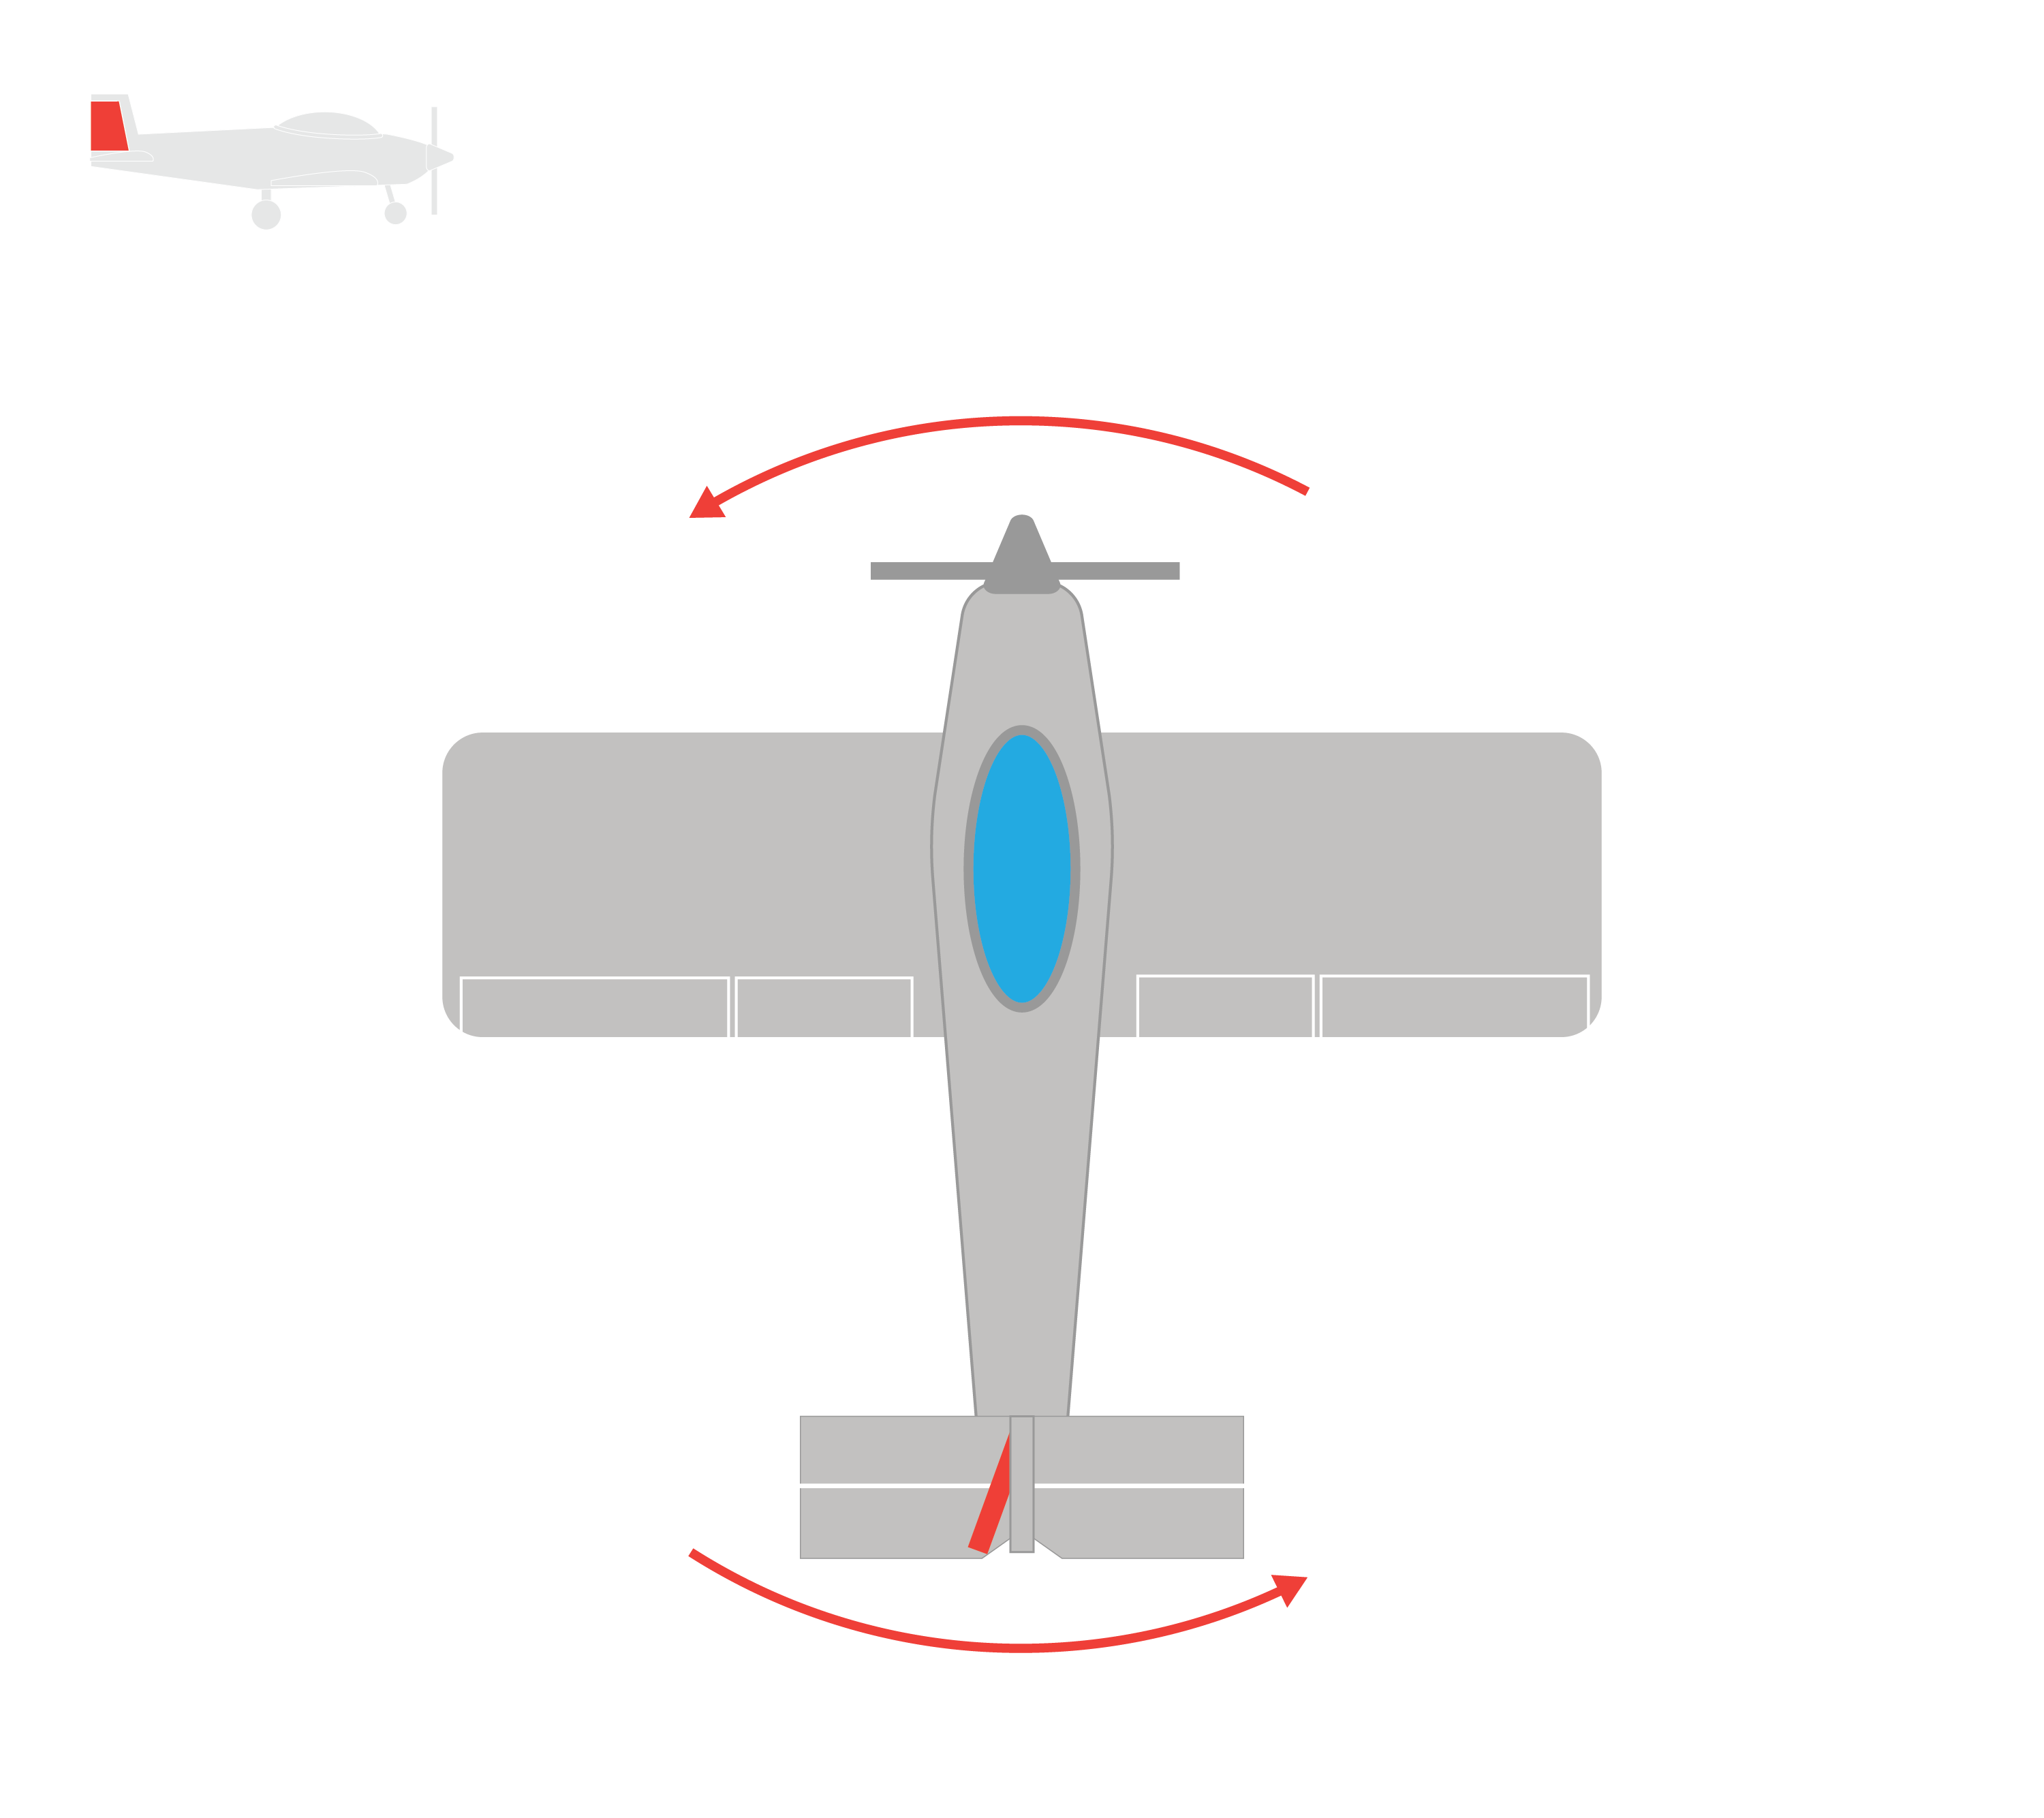
\includegraphics[width=0.55\textwidth]{rudder.png}
  \caption{The rudder controls yaw, the left-right swing of the nose.}\label{fig:rudderYaw}
\end{figure}

\index{flaps}\newterm{Flaps} are panels on the back edges of the wings. For
takeoff and landing, the pilot extends them down, which gives the wings
more lift (and more drag) at low speeds.

\begin{figure}[H]
  \centering
  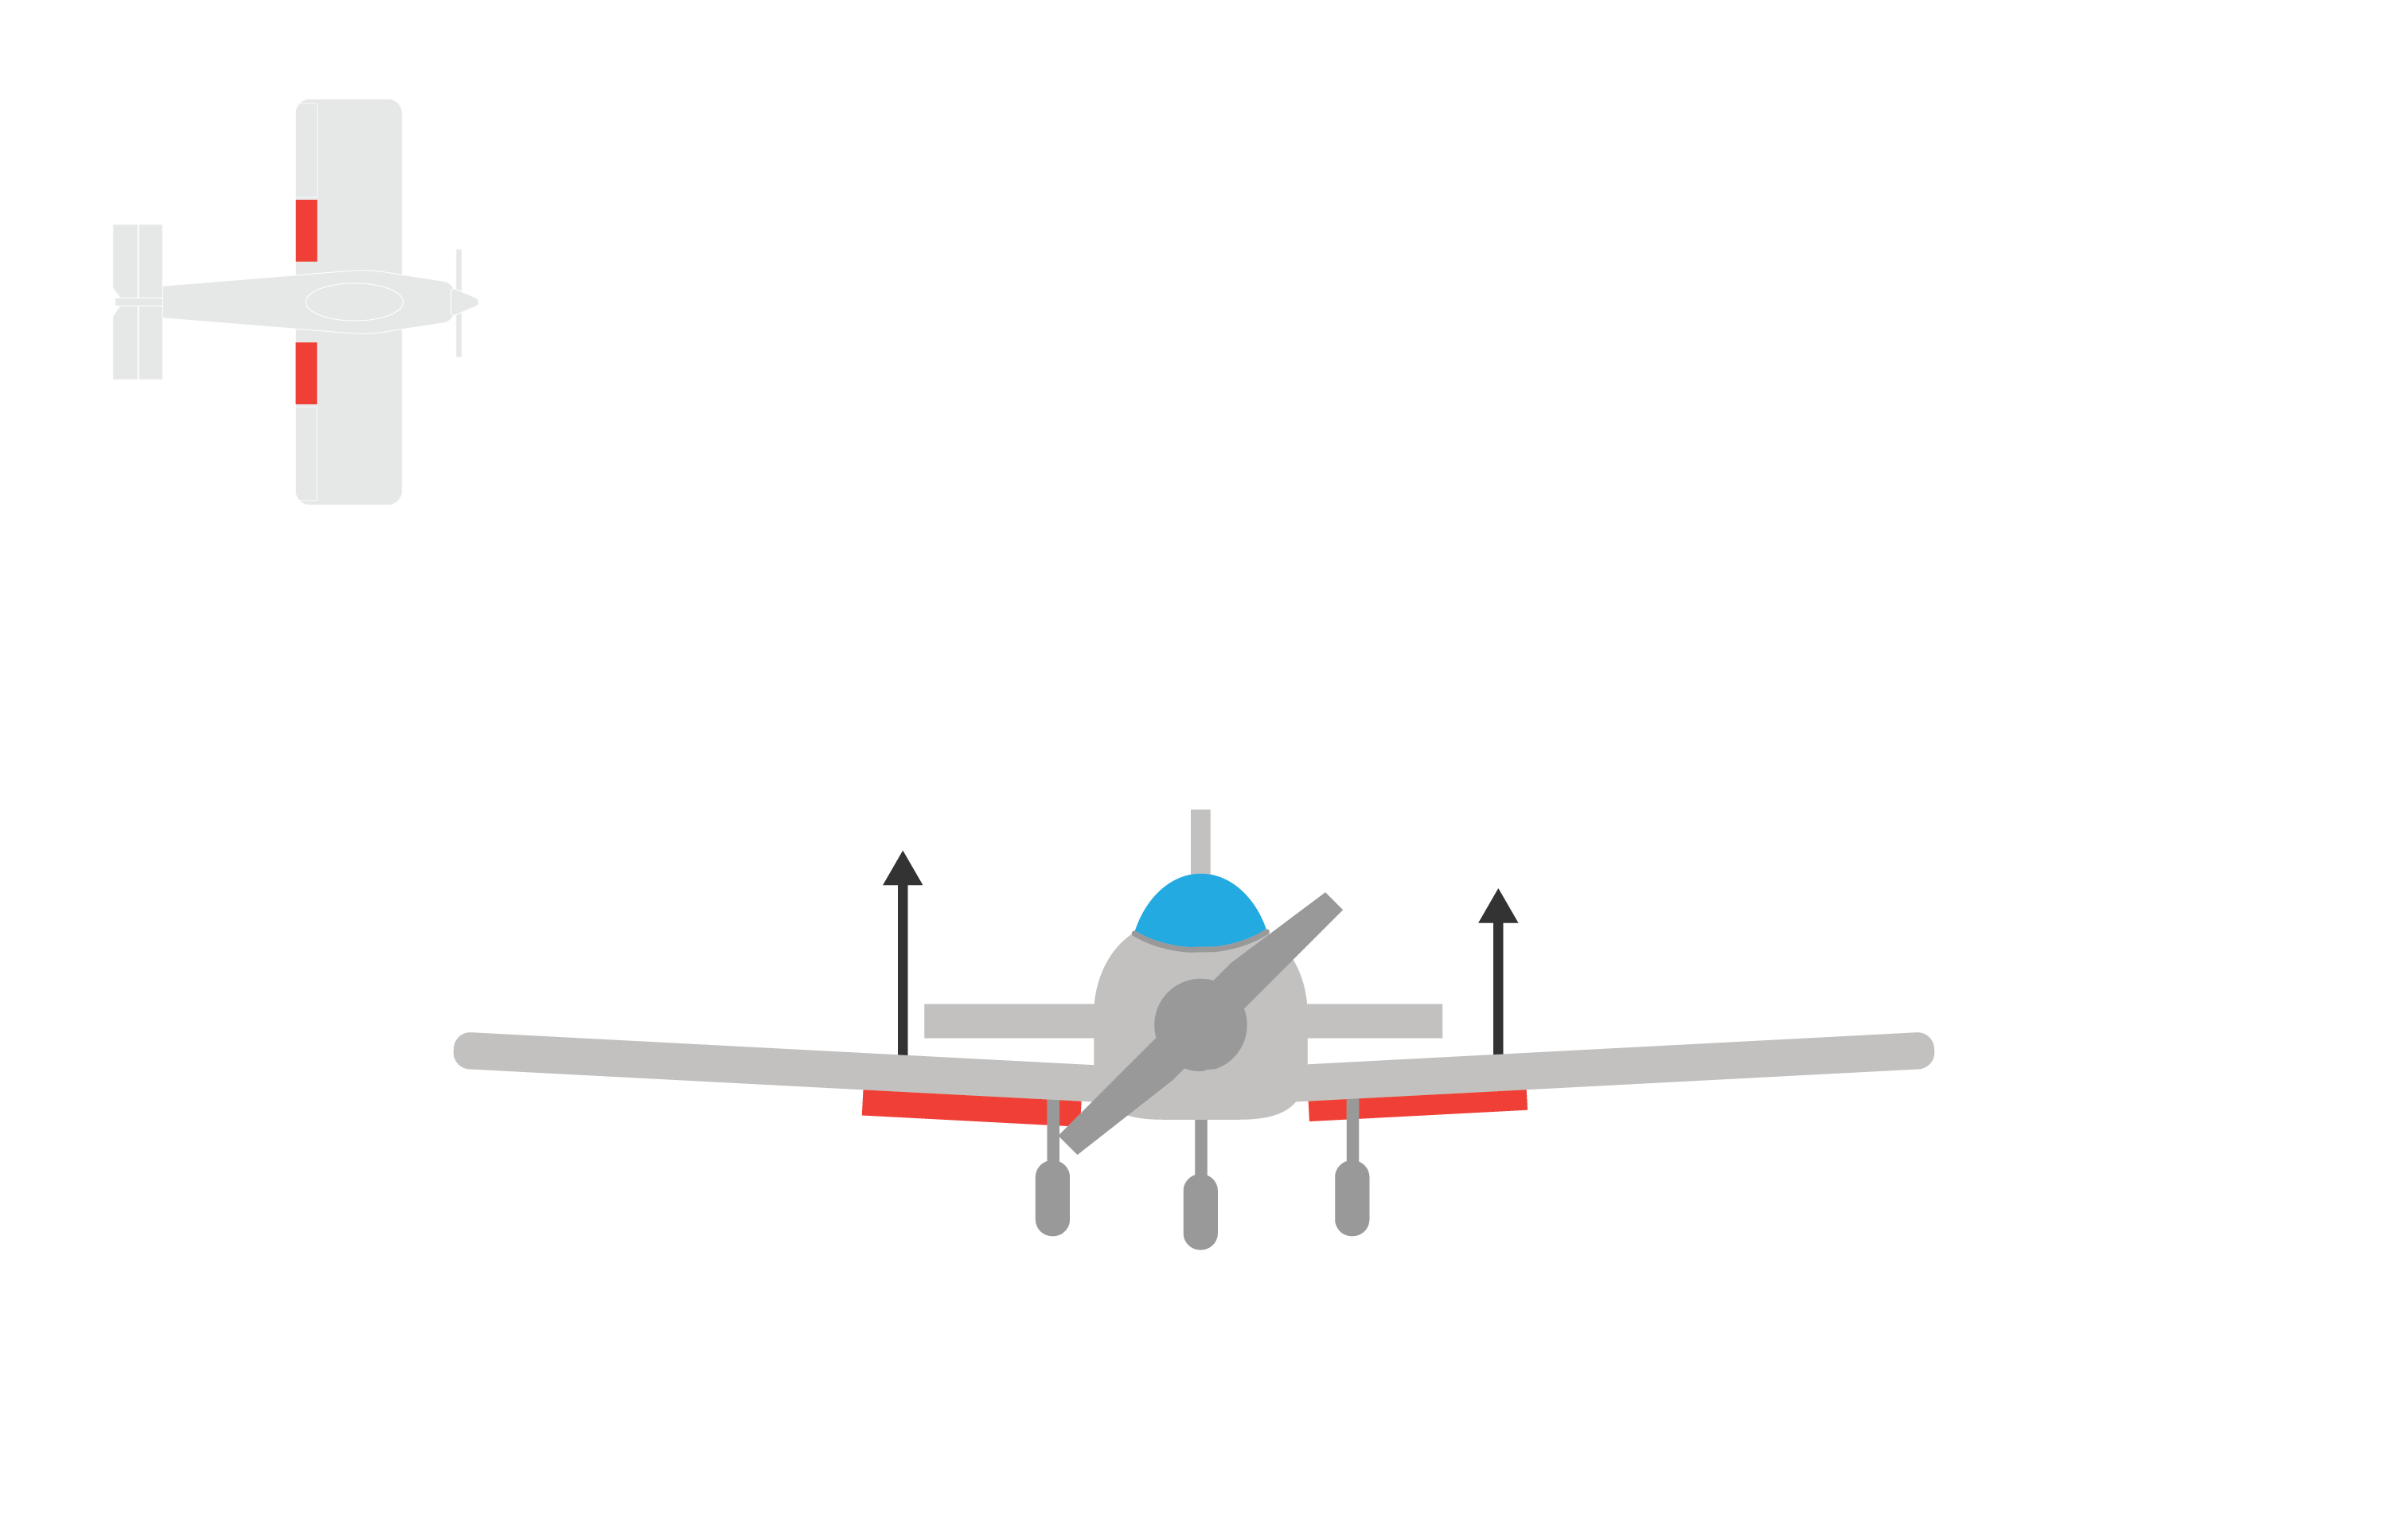
\includegraphics[width=0.55\textwidth]{flaps.png}
  \caption{The location and effect of the flaps.}\label{fig:flaps}
\end{figure}

\section{Thrust}

There are three common ways to make thrust.

A \newterm{propeller} is a spinning set of small wings. Each blade is an
airfoil turned on its side, so its ``lift'' points forward. Small planes
spin their propellers with piston engines much like car engines.
\begin{figure}[H]
  \centering
  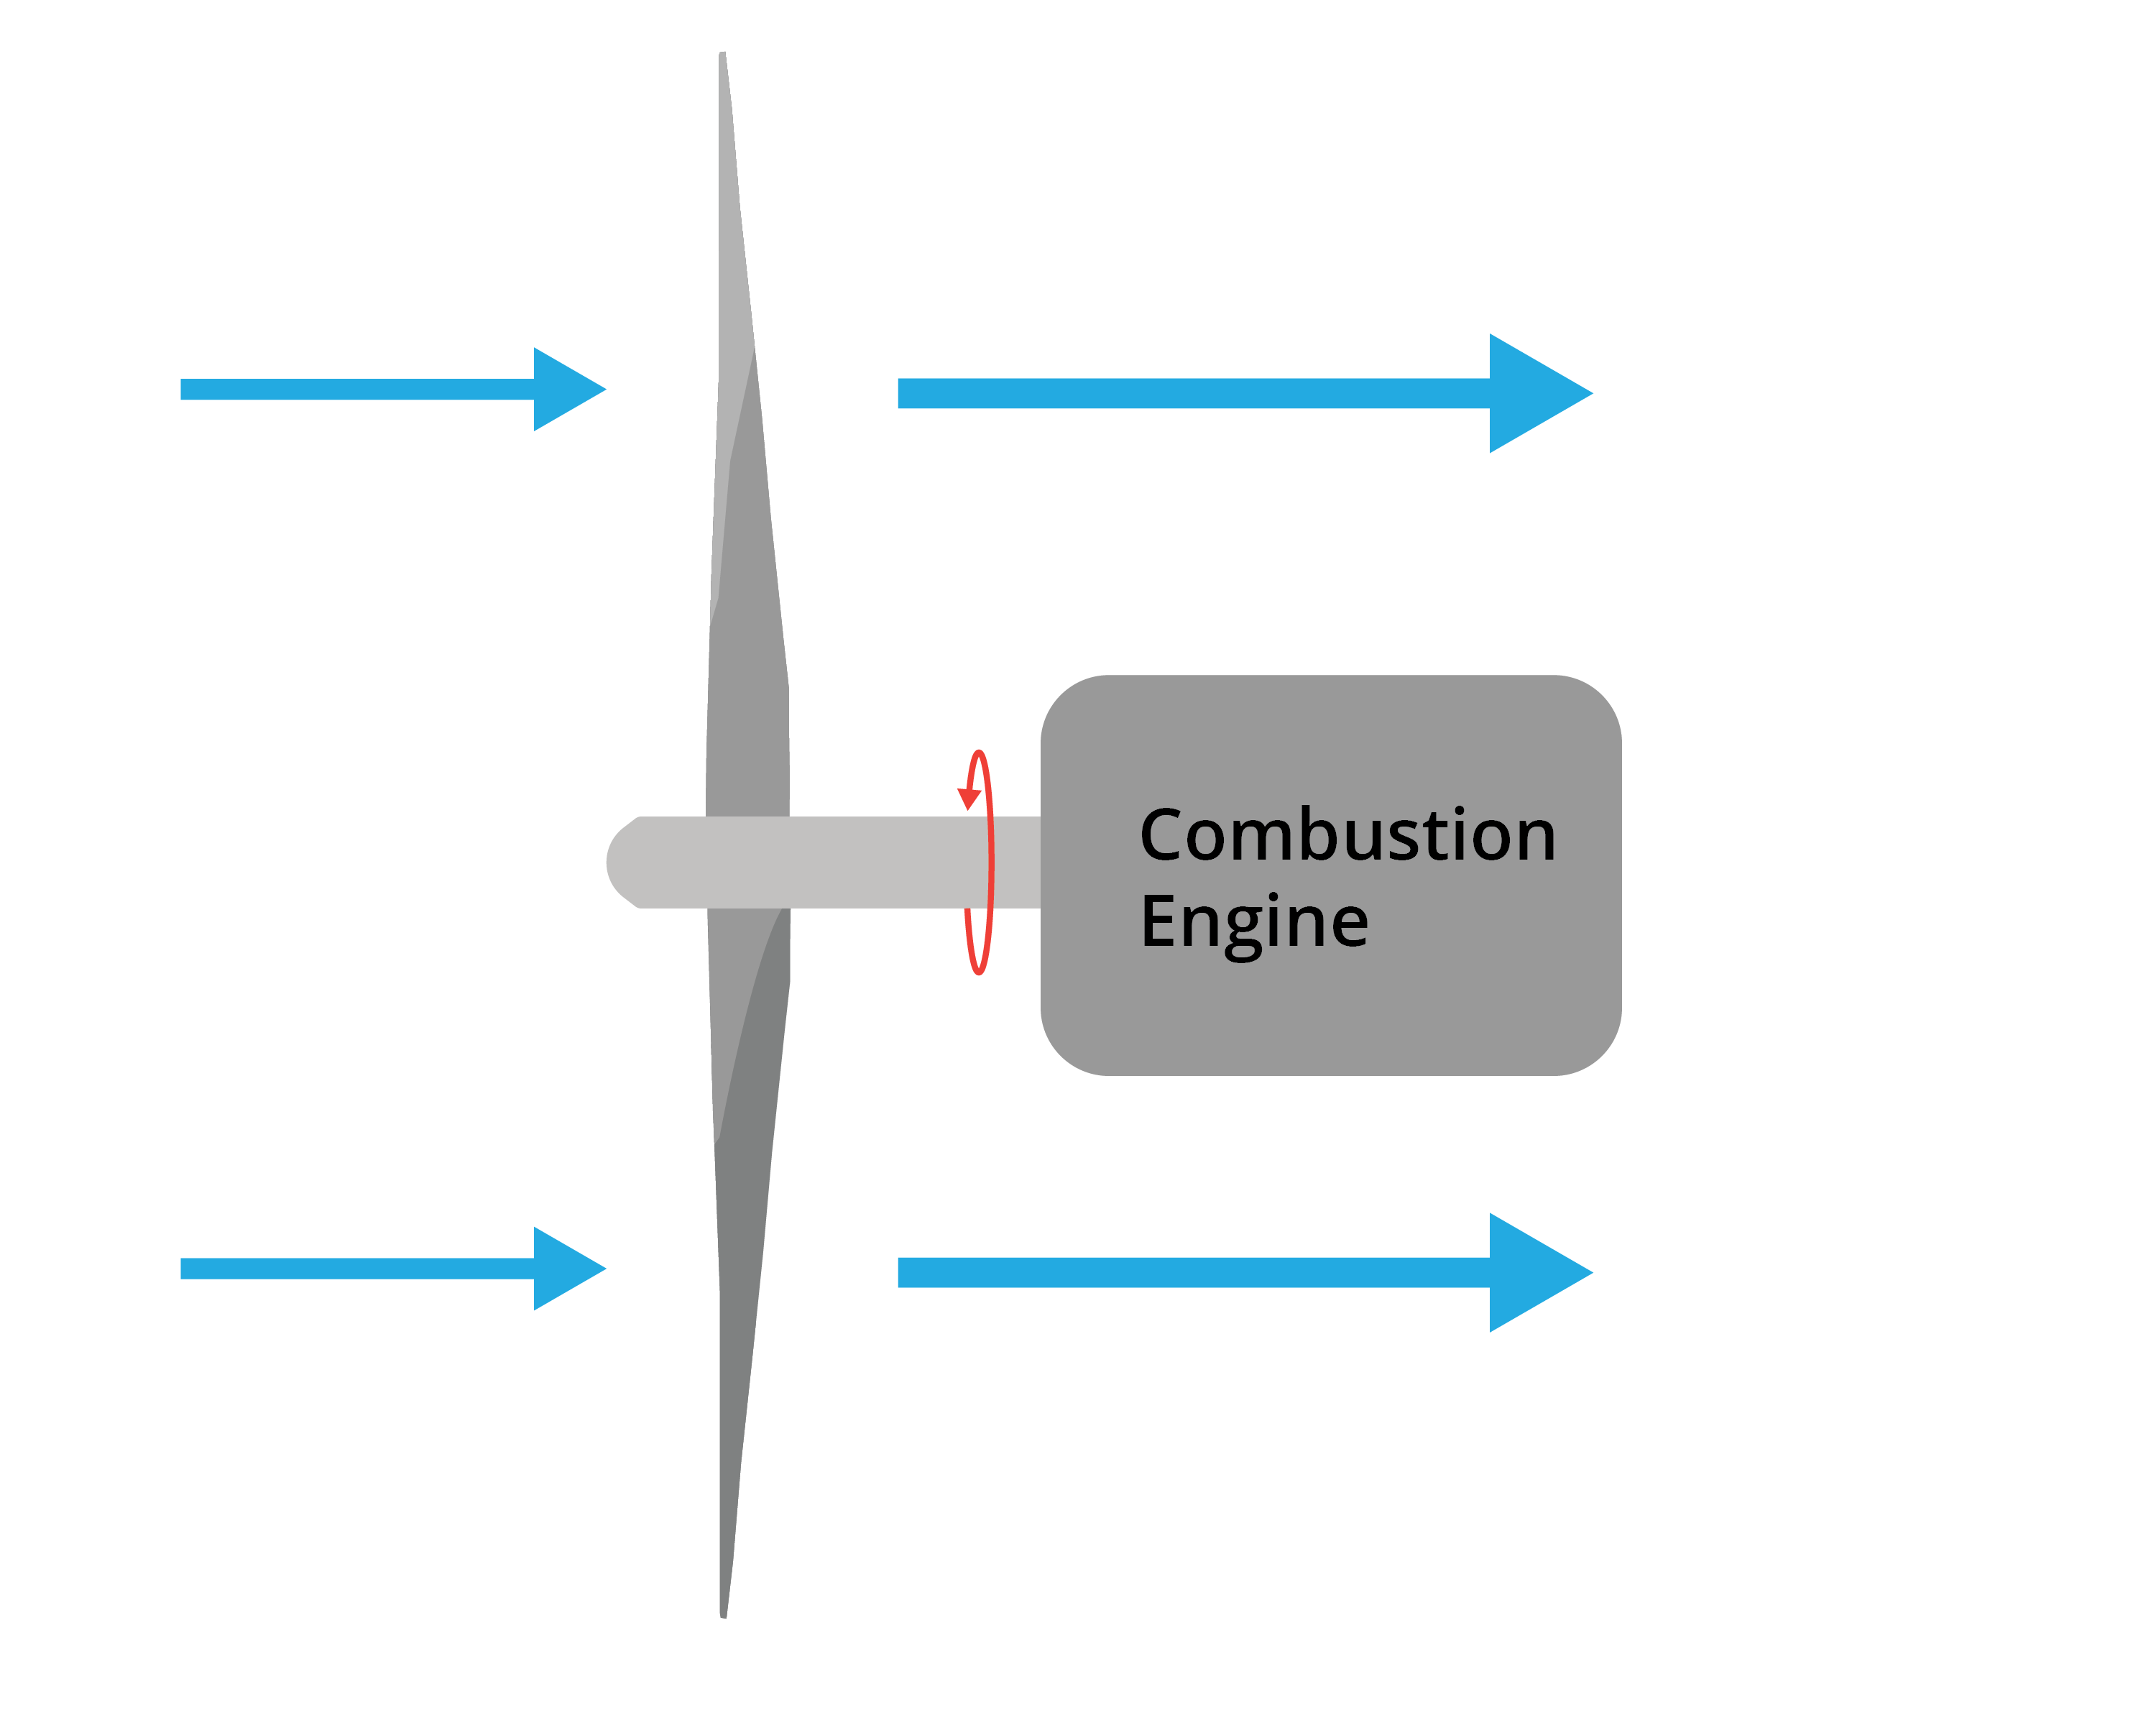
\includegraphics[width=0.55\textwidth]{propeller.png}
  \caption{Each propeller blade is a small spinning wing whose lift points forward.}\label{fig:propeller}
\end{figure}

\index{jet engine}A \newterm{jet engine} sucks in air, squeezes it with a
spinning compressor, sprays in fuel, and burns the mixture. The hot gas
roars out the back much faster than the air came in, and that pushes the
plane forward. On its way out, the gas spins a turbine, which drives the
compressor at the front.

\begin{figure}[H]
  \centering
  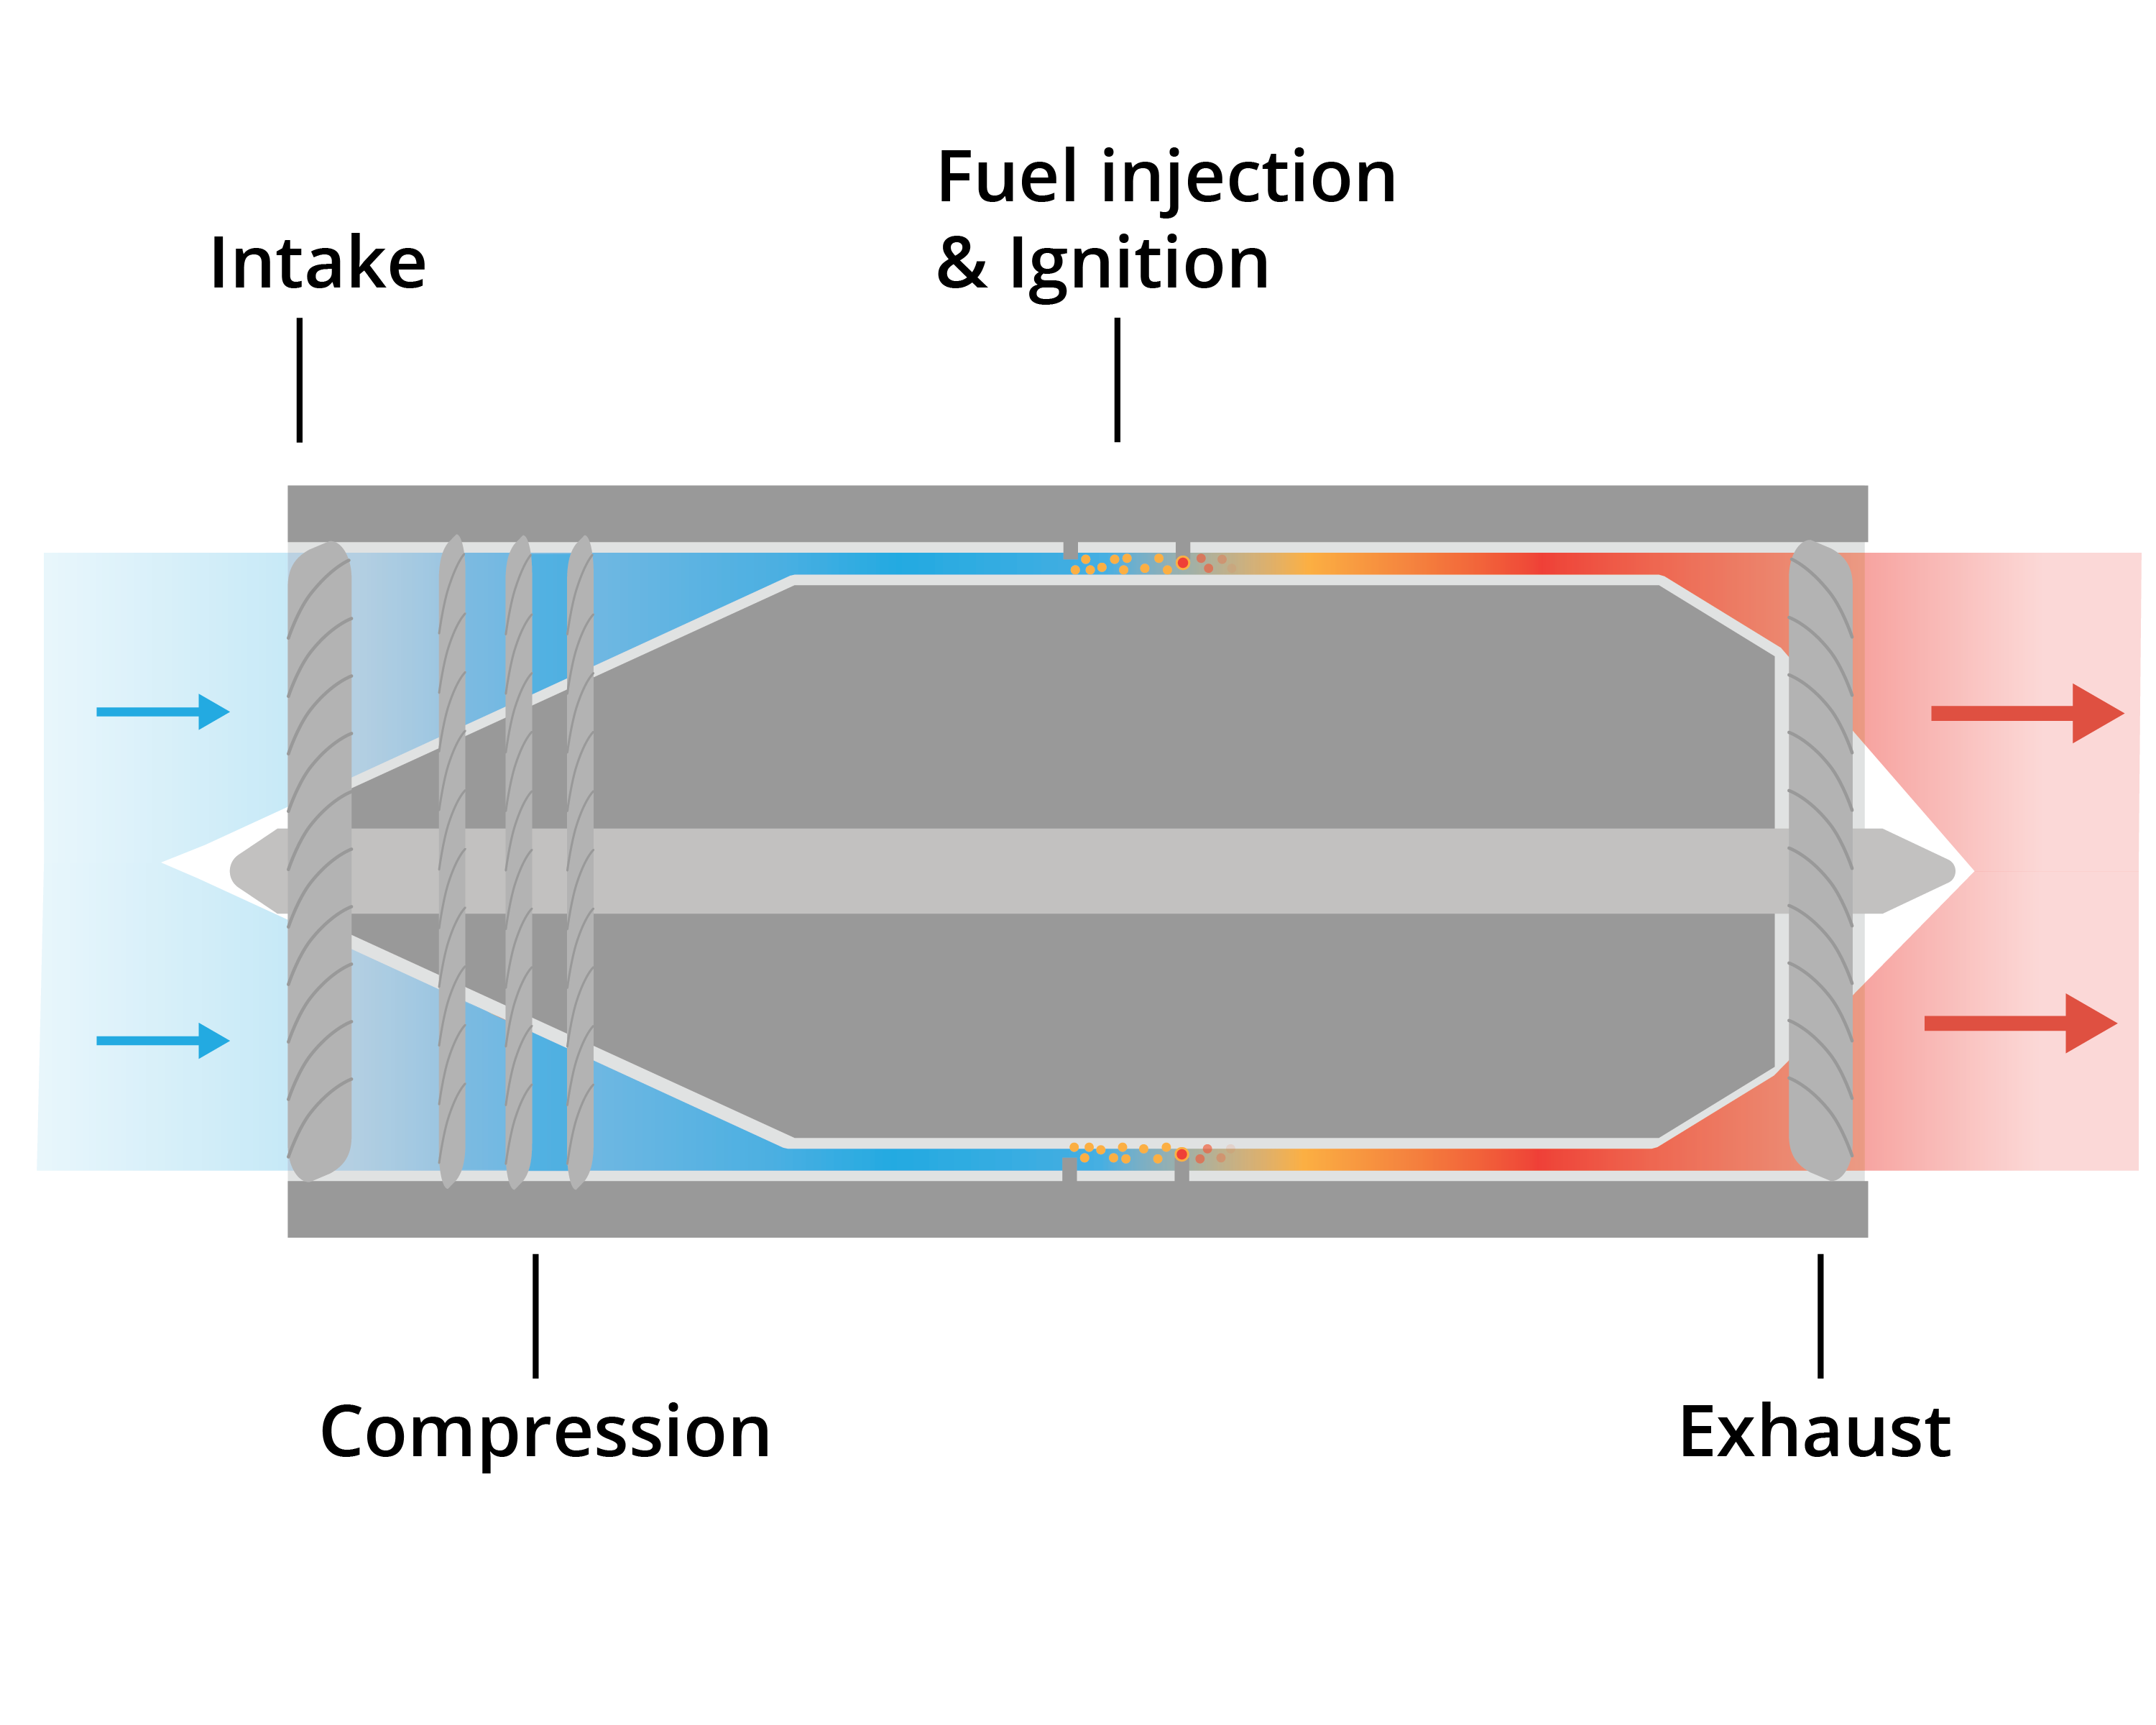
\includegraphics[width=0.55\textwidth]{jet.png}
  \caption{Cross section of a jet engine.}\label{fig:jet}
\end{figure}

A \newterm{turboprop} uses a jet engine's turbine to spin a propeller.
Turboprops are efficient at the lower speeds and shorter hops flown by
regional airlines.

\begin{figure}[H]
  \centering
  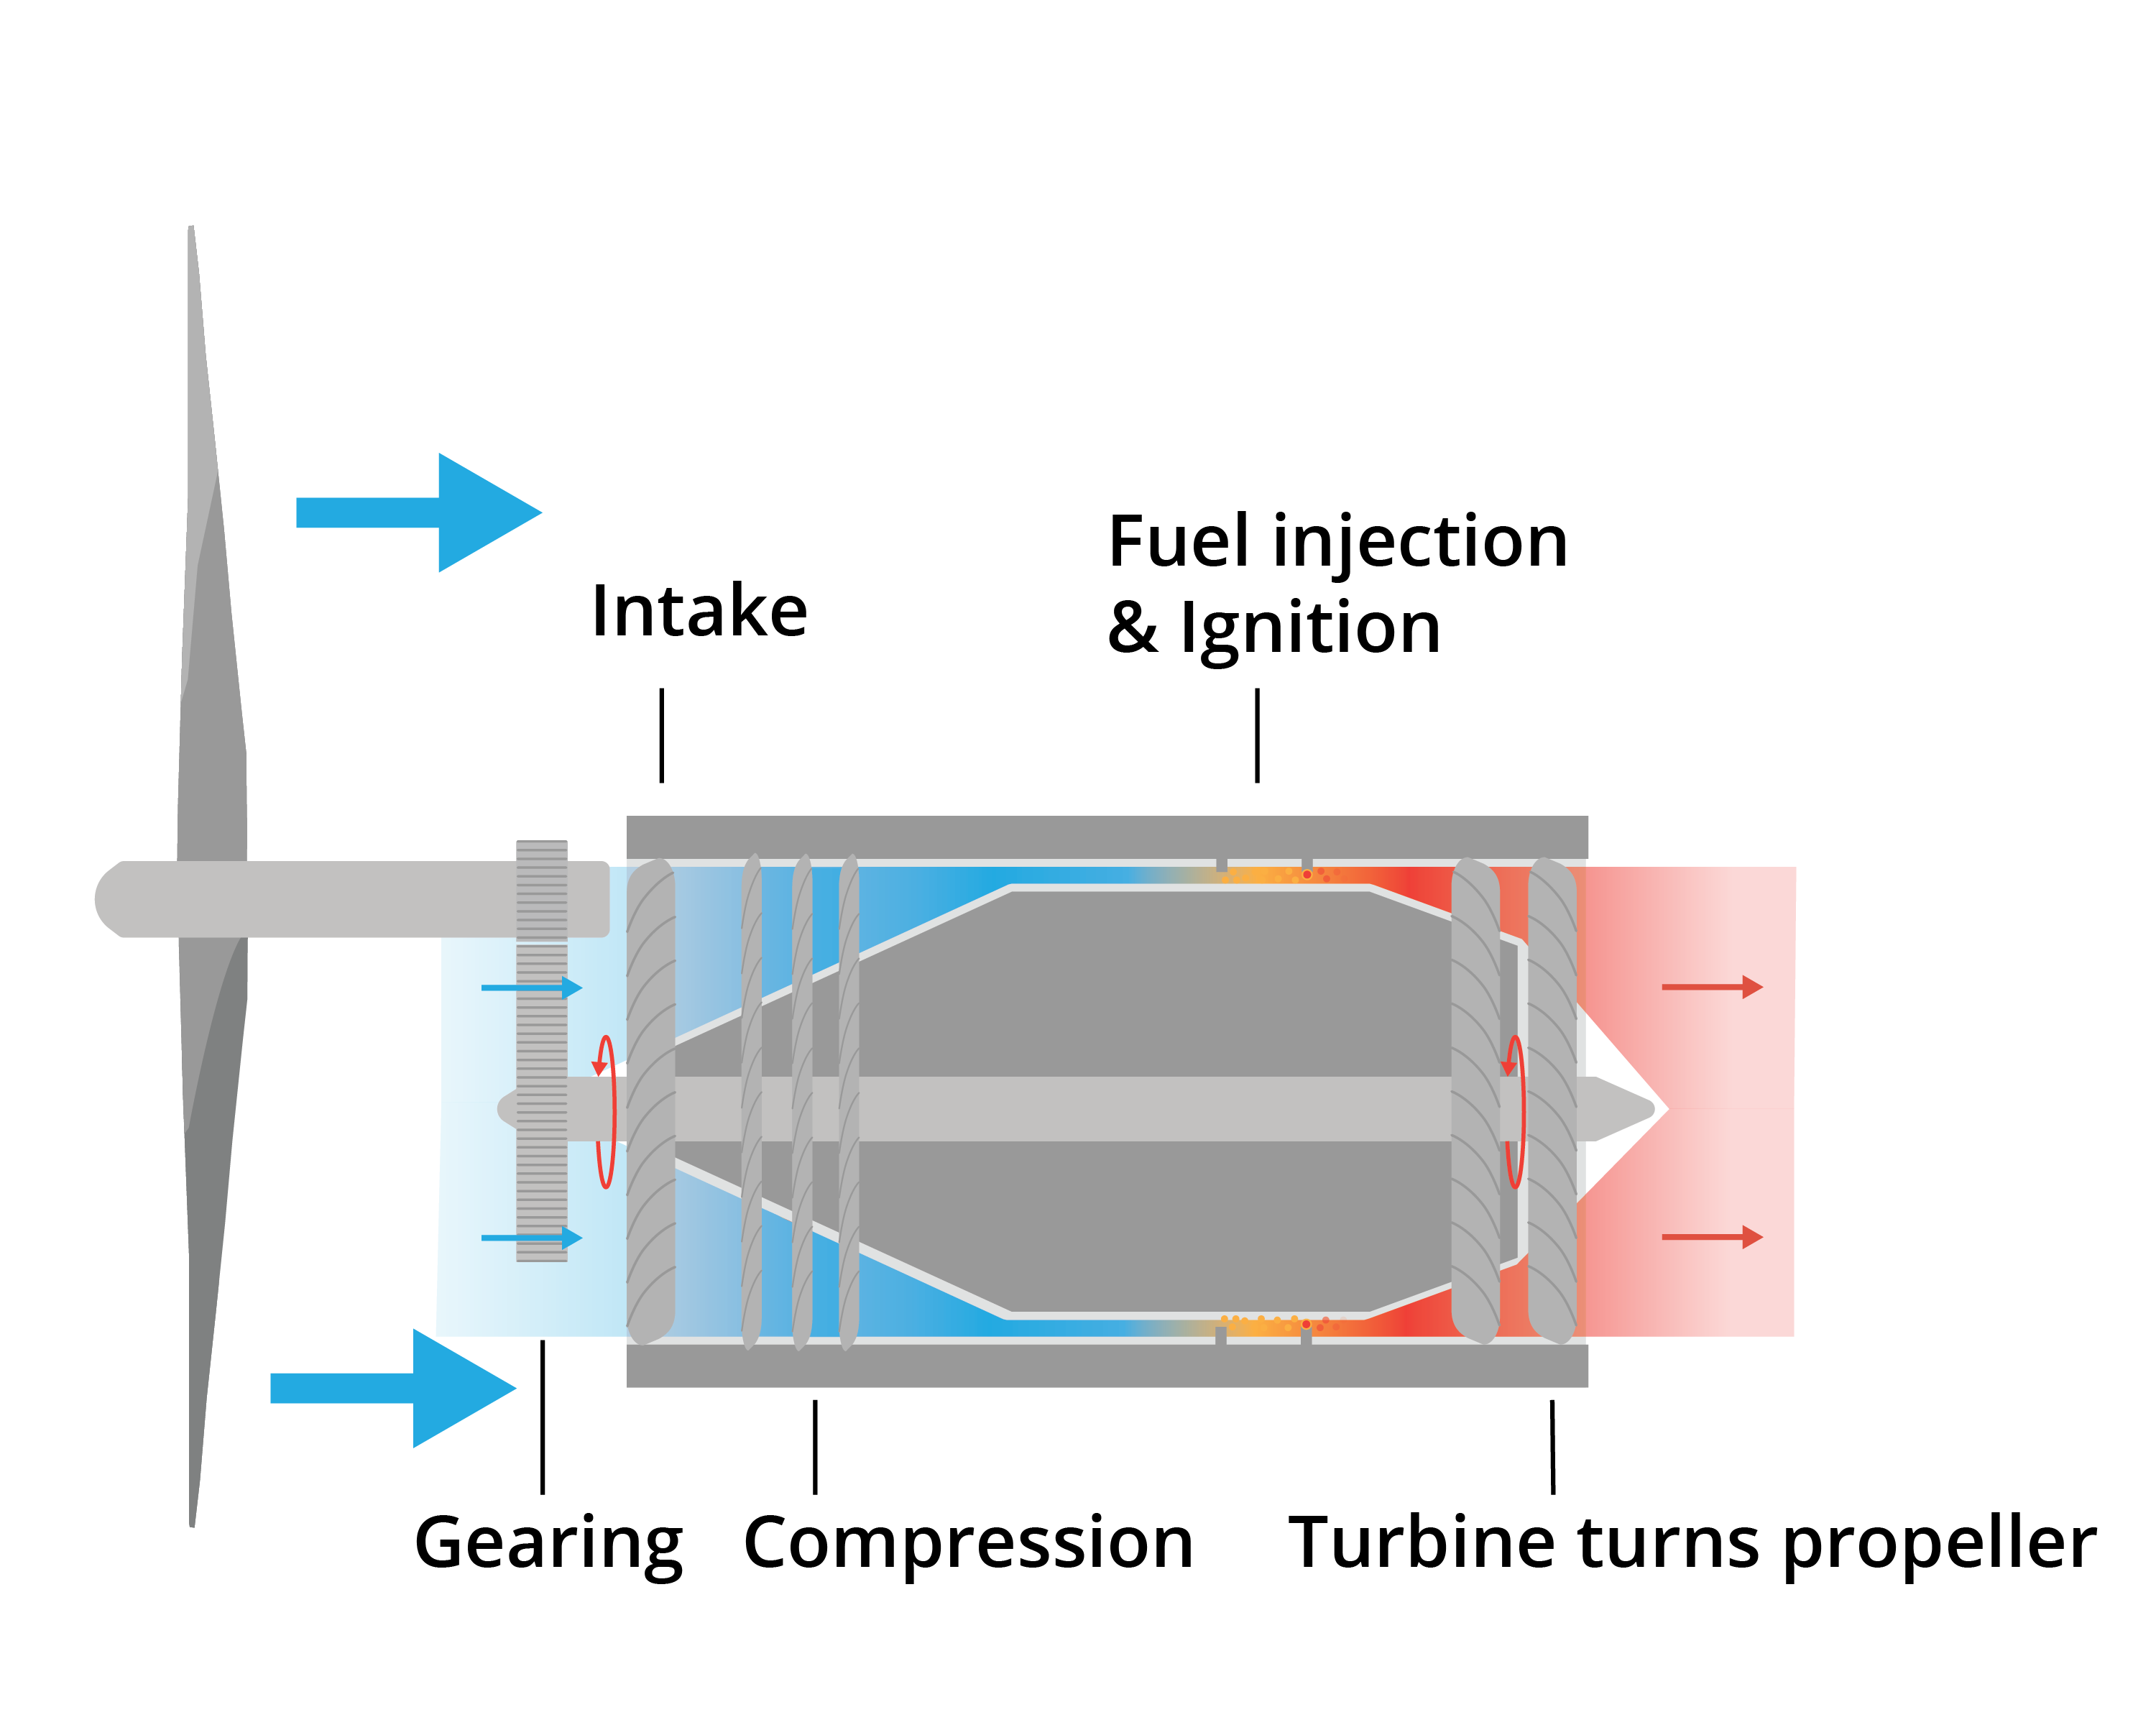
\includegraphics[width=0.55\textwidth]{turboProp.png}
  \caption{Cross section of a turboprop.}\label{fig:turboProp}
\end{figure}

\section{Gliders}
\index{gliders}

A glider has no engine at all. It starts high in the air with lots of
potential energy and trades height for speed, sliding gently downhill
through the air. A good glider can travel 40 meters forward for every meter
it descends; this is its \newterm{glide ratio}. To stay up for hours, glider
pilots hunt for rising air, such as warm air rising from a sunny parking
lot, and circle in it to regain height.

\begin{Exercise}[title={How far can it glide?}, label=fl_glide]
A glider with a glide ratio of 40 is released at an altitude of 1,500 m.
In still air, how far can it glide before it reaches the ground?
\end{Exercise}
\begin{Answer}[ref=fl_glide]
$40 \times 1{,}500 = 60{,}000$ m, or 60 km.
\end{Answer}

Airplanes need runways and a steady stream of air over their wings. The next chapter, Drones, Helicopters,
and Rockets, looks at machines that can hover, and at machines that fly where there is no air at all.
